\documentclass[journal]{IEEEtran}

% ---------------------------------------------------------------------------
% Paquetes
% ---------------------------------------------------------------------------
\usepackage[utf8]{inputenc}
\usepackage[T1]{fontenc}
\usepackage[spanish,es-nodecimaldot]{babel}
\usepackage{graphicx}
\usepackage{amsmath,amssymb,amsthm}
\usepackage{booktabs}
\usepackage{tabularx}
\usepackage{array}
\usepackage{multirow}
\usepackage{multicol}
\usepackage{xcolor}
\usepackage{caption}
\usepackage{subcaption}
\usepackage{hyperref}
\usepackage{url}
\usepackage{cite}
\usepackage{tikz}
\usetikzlibrary{arrows.meta,positioning,fit,calc}

\graphicspath{{figuras/}}

% ---------------------------------------------------------------------------
% Metadatos
% ---------------------------------------------------------------------------
\hypersetup{
  pdftitle={Clasificación multietiqueta de discurso de odio, carácter dirigido y agresividad en tuits en español mediante TF-IDF y ensambles lineales},
  pdfauthor={Rivera Jiménez, Carrillo Meneses, Garnica Salazar y Prieto Moreno},
  pdfsubject={Clasificación multietiqueta de discurso de odio},
  hidelinks
}

\renewcommand{\abstractname}{Resumen}
\renewcommand{\IEEEkeywordsname}{Palabras clave}
\renewcommand{\appendixname}{Apéndice}
\addto\captionsspanish{\renewcommand{\tablename}{Tabla}}

\newtheorem{proposicion}{Proposición}

% ---------------------------------------------------------------------------
% Documento
% ---------------------------------------------------------------------------
\begin{document}

\title{Clasificación multietiqueta de discurso de odio, carácter dirigido y
agresividad en tuits en español mediante TF-IDF y ensambles lineales}

\author{
\IEEEauthorblockN{Erika Valeria Rivera Jiménez\IEEEauthorrefmark{1},
Julián Guillermo Carrillo Meneses\IEEEauthorrefmark{1},
Carlos Andrés Garnica Salazar\IEEEauthorrefmark{1} y
Oscar Andrés Prieto Moreno\IEEEauthorrefmark{1}}\\
\IEEEauthorblockA{\IEEEauthorrefmark{1}Pontificia Universidad Javeriana,
Bogotá, Colombia\\
Maestría en Inteligencia Artificial --- Procesamiento de Lenguaje Natural\\
\url{riveraev@javeriana.edu.co}, \url{carrillojuliang@javeriana.edu.co},\\
\url{carlos_garnicas@javeriana.edu.co}, \url{o-prieto@javeriana.edu.co}}
}

\maketitle

\begin{abstract}
La detección automática de discurso de odio en español es una tarea
multietiqueta: un mismo tuit puede ser odioso, estar dirigido contra una
persona o grupo y ser agresivo, y las tres decisiones no son independientes.
Este artículo documenta el diseño, la experimentación y la validación del
sistema presentado a la competencia académica \emph{TOXIC 2026 PUJ}, sujeta a
una restricción severa: prohibido usar transformers, modelos de lenguaje o
embeddings preentrenados; las representaciones debían entrenarse desde cero.
Sobre 1\,731 tuits de entrenamiento y 1\,154 sin etiquetas, construimos una
representación subléxica multiescala de 86\,275 características TF-IDF, un
ensamble de tres optimizadores lineales con calibración de temperatura,
umbrales desacoplados por etiqueta y la regla ontológica de HatEval. La
validación cruzada agrupada, que fusiona near-duplicados y pseudo-autores,
sitúa al modelo base en 0.787582 out-of-fold, con una mejora de $+0.010370$
sobre la línea base (IC95 $[+0.003924, +0.017386]$). Una capa de decisión de
pares compensados, que preserva la prevalencia predicha y se calibra con el
leaderboard público, eleva el $F_1$ público a 0.81447, primer lugar al cierre
de este informe. El artículo separa el modelo base, validado estadísticamente,
de la capa de última milla, específica del test, y discute su riesgo de
sobreajuste. El envío se reconstruye bit a bit (SHA256
\texttt{b0979a8a\ldots}), con dos celdas de frontera fijadas y auditadas; dos
ejecuciones independientes producen el mismo archivo.
\end{abstract}

\begin{IEEEkeywords}
detección de discurso de odio, clasificación multietiqueta, representación
subléxica, TF-IDF, calibración de umbrales, validación agrupada,
reproducibilidad.
\end{IEEEkeywords}

% Ajuste de espaciado de flotantes para consolidar la maquetacion
\setlength{\textfloatsep}{6pt plus 1.0pt minus 2.0pt}
\setlength{\floatsep}{5pt plus 1.0pt minus 2.0pt}
\setlength{\intextsep}{5pt plus 1.0pt minus 2.0pt}

\section{Introducción}
\label{sec:introduccion}

La conversación pública en redes sociales plantea un problema de clasificación
que no admite una lectura ingenua: el discurso de odio rara vez aparece
aislado. En un mismo tuit conviven la deshumanización de un grupo, la
agresión explícita y el señalamiento de una persona concreta. Los corpus
anotados para la tarea lo reflejan: en HatEval, por ejemplo, las etiquetas de
discurso de odio (\emph{hate speech}, HS), carácter dirigido (\emph{targeted},
TR) y agresividad (AG) se anotan de forma conjunta y condicionada
\cite{basile2019hateval}. Modelar las tres columnas como decisiones
independientes ignora esa estructura; modelarlas como una única clase de seis
combinaciones pierde la señal compartida y multiplica la escasez de cada
celda. La formulación multietiqueta, con un clasificador por etiqueta y una
regla ontológica que preserva la jerarquía, es el compromiso que adoptamos
aquí.

El contexto de este trabajo es la competencia académica \emph{TOXIC 2026 PUJ},
organizada para el curso de Procesamiento de Lenguaje Natural de la Maestría
en Inteligencia Artificial de la Pontificia Universidad Javeriana. La
competencia impone tres restricciones fundamentales: (i) prohibición de
utilizar arquitecturas basadas en transformers o modelos de lenguaje; (ii)
obligación de entrenar todas las representaciones desde cero a partir del
conjunto de entrenamiento; y (iii) prohibición de emplear el conjunto de
prueba para el ajuste del modelo base (la calibración de la capa de decisión
se guía únicamente por la retroalimentación agregada del leaderboard público). La métrica oficial es la media columnar de la $F_1$ binaria
de la clase positiva sobre HS, TR y AG \cite{opitz2019macro}. La nota final
combina el leaderboard privado con la claridad y justificación del cuaderno
entregado, de modo que el resultado y su explicación pesan por igual.

La pregunta que organiza este artículo es directa: \emph{¿puede un pipeline
clásico, sin transformers ni representaciones preentrenadas, competir en un
corpus pequeño y ruidoso de tuits en español?} La respuesta que documentamos
es afirmativa, pero con una distinción que consideramos central. El modelo
base ---representación subléxica, ensamble lineal y umbrales desacoplados---
alcanza un $F_1$ out-of-fold de 0.787582 y una mejora estadísticamente
sostenida sobre la línea base. La capa de decisión de última milla ---reglas
de staging y pares compensados--- eleva el leaderboard público hasta 0.81447,
pero lo hace con intervenciones específicas del test, guiadas por el propio
leaderboard. Separar ambas fuentes de mejora, en lugar de presentar el
0.81447 como si fuera una estimación limpia de generalización, es una de las
contribuciones metodológicas del trabajo.

Las contribuciones concretas son cinco. Primera, un pipeline clásico
completo y reproducible: una representación TF-IDF multiescala de 86\,275
características, un ensamble de tres optimizadores lineales con calibración
de temperatura y umbrales por etiqueta. Segunda, un protocolo de validación
agrupada que fusiona near-duplicados y pseudo-autores, verifica la ausencia
de fuga en cada pliegue y se replica en dos particiones congeladas. Tercera,
un análisis formal de la capa de decisión: demostramos que un par compensado
que rescata un verdadero positivo y suprime un falso positivo en la misma
columna incrementa la $F_1$ exactamente en $F_1/TP$, sin alterar el número de
positivos. Cuarta, una descomposición explícita de la ganancia del
leaderboard en sus dos componentes y una discusión de su validez externa.
Quinta, un contrato de reproducibilidad verificado: el envío campeón se
reconstruye bit a bit y dos ejecuciones independientes producen el mismo
archivo.

El resto del artículo sigue el orden de CRISP-DM. La
Sección~\ref{sec:trabajos} sitúa el trabajo frente a la literatura
(comprensión del negocio y estado del arte). La Sección~\ref{sec:datos}
describe el corpus y el análisis exploratorio (comprensión de los datos). La
Sección~\ref{sec:metodologia} detalla la preparación, la representación, los
modelos y la capa de decisión. La Sección~\ref{sec:resultados} recorre los
veinticinco experimentos evaluados en el leaderboard y separa lo que funcionó
de lo que no (modelado). La Sección~\ref{sec:discusion} presenta el análisis
estadístico, el análisis de error y los límites del enfoque (evaluación). La
Sección~\ref{sec:reproducibilidad} documenta el despliegue y la verificación
criptográfica. La Sección~\ref{sec:conclusiones} cierra con las lecciones y
el trabajo futuro.

Por convención numérica, y para no alterar los identificadores del registro
oficial de Kaggle, en todo el artículo se usa el punto como separador decimal
y el espacio fino para los miles.

\section{Trabajos relacionados}
\label{sec:trabajos}

\subsection{Detección de discurso de odio y la herencia de HatEval}

La detección de discurso de odio es una tarea consolidada en el procesamiento
del lenguaje natural, con revisiones sistemáticas que cubren definiciones,
corpus y enfoques \cite{schmidt2017survey,fortuna2018survey,jahan2023systematic}.
Un hito para el español y el multilingüismo fue la tarea 5 de SemEval-2019
(HatEval), que introdujo la anotación conjunta de odio y carácter dirigido
contra inmigrantes y mujeres \cite{basile2019hateval}. Los sistemas
participantes combinaron rasgos lingüísticos, n-gramas de caracteres y modelos
lineales o neuronales \cite{argotavega2019mineriaunam,ninaalcocer2019haterecognizer,plazadelarco2019sinai}.
La lección que heredamos es doble: la estructura de las etiquetas importa y
los corpus son pequeños, ruidosos y sensibles al dominio.

En español, HaterNet mostró que un clasificador lineal sobre representaciones
dispersas podía competir con alternativas más complejas en un corpus de
Twitter \cite{pereirakohatsu2019haternet}; MexA3T exploró la agresividad y el
odio en variantes del español de México \cite{alvarezcarmona2018mexa3t,aragon2019mexa3t};
otros trabajos abordaron la misoginia y la combinación de rasgos lingüísticos
\cite{garcia2021misogyny,garcia2022featurecombination,frenda2018misogyny,arango2019hate}.
Los transformers han elevado el techo en corpus grandes
\cite{plazadelarco2021comparing,plazadelarco2021multitask}, pero su ventaja se
reduce cuando el corpus es pequeño, el dominio está normalizado y el
presupuesto de cómputo es limitado. La restricción de esta competencia
---sin modelos preentrenados--- vuelve relevante la pregunta inversa: cuánto
se puede extraer de una representación construida desde cero.

\subsection{Representaciones subléxicas y modelos lineales}

Los n-gramas de caracteres son una representación clásica para texto corto y
ruidoso. Cavnar y Trenkle los usaron para categorización de texto
\cite{cavnar1994ngram} y McNamee y Mayfield mostraron su eficacia en
recuperación multilingüe \cite{mcnamee2004character}. La representación
TF-IDF \cite{salton1988term} combinada con regresión logística o máquinas
de vectores sigue siendo una línea base difícil de superar en corpus
pequeños. Los optimizadores importan: \textsc{liblinear} resuelve el problema
primal con coordenadas \cite{fan2008liblinear}, el descenso estocástico
escala a matrices dispersas \cite{bottou2010large} y SAGA acelera la
regularización ElasticNet \cite{defazio2014saga,zou2005regularization}. Los
ensambles de modelos diversos ---bagging, stacking o mezclas de
probabilidades--- reducen varianza y suavizan los errores de frontera
\cite{breiman1996bagging,wolpert1992stacked}. Nuestra propuesta se sitúa en
esa tradición, pero añade una capa de decisión explícita y auditable.

\subsection{Umbrales, calibración y estructura de etiquetas}

En clasificación desbalanceada, el umbral de 0.5 no es óptimo para la $F_1$
\cite{japkowicz2002class,lipton2014thresholding}. La literatura ofrece
soluciones analíticas y numéricas para maximizar la $F_1$ por clase
\cite{nan2012optimizing,dembczynski2013optimizing,parambath2014optimizing,berger2020threshold}
y advierte que la métrica tiene una geometría propia: no todas las celdas de
la matriz de confusión pesan igual \cite{flach2003geometry,saito2015precision}.
La calibración de probabilidades es el paso previo: la temperatura y el
escalado de Platt corrigen el exceso de confianza de los modelos
\cite{guo2017calibration,platt1999probabilistic}. Finalmente, la estructura
jerárquica de las etiquetas ---TR solo tiene sentido si HS está activo---
puede explotarse con reglas ontológicas o con clasificadores jerárquicos
\cite{silla2011survey,fortuna2019hierarchically}. Nuestro pipeline combina
las tres ideas: calibración, umbrales desacoplados y una regla ascendente.

\subsection{Calidad de datos, fuga y comparación estadística}

Los corpus de odio contienen near-duplicados, retuits, hilos de un mismo
usuario y etiquetas ambiguas \cite{founta2018crowdsourcing,davidson2017automated,davidson2019racial,wiegand2019biased}.
Si la validación reparte copias casi idénticas entre entrenamiento y
validación, la métrica local se infla: es la fuga por agrupamiento descrita
por Kaufman et al. \cite{kaufman2012leakage}. La respuesta metodológica es
agrupar antes de partir y verificar que ningún grupo cruce la frontera
\cite{kohavi1995study,kaufman2012leakage}. La comparación entre modelos
tampoco debería apoyarse en una única diferencia de medias: el bootstrap
agrupado, las pruebas pareadas de McNemar y los tests de Dietterich y Demšar
son el estándar para decidir si una mejora es distinguishable del ruido
\cite{efron1979bootstrap,mcnemar1947note,dietterich1998approximate,demsar2006statistical}.
Ese es el marco que adoptamos.

\subsection{Posicionamiento}

Este trabajo no propone una arquitectura nueva. Propone una \emph{disciplina}
de construcción y evaluación: representación subléxica multiescala,
validación agrupada, umbrales por etiqueta, calibración y una capa de
decisión que preserva la prevalencia. La contribución diferencial es el
análisis formal de esa capa y la separación explícita entre lo que se valida
localmente y lo que se ajusta contra el leaderboard. Frente a los sistemas
basados en transformers, el nuestro es más simple y más barato; frente a las
líneas base clásicas, incorpora una ingeniería de decisión que resulta
decisiva en la competencia.

\section{Datos y análisis exploratorio}
\label{sec:datos}

\subsection{Corpus e integridad}

El corpus de la competencia contiene 1\,731 tuits etiquetados para
entrenamiento y 1\,154 sin etiquetas de prueba. Cada fila de entrenamiento tiene un
identificador, el texto y tres columnas binarias: HS (discurso de odio), TR
(carácter dirigido) y AG (agresividad). La auditoría de integridad verifica
que no hay valores nulos, que los identificadores son únicos y que se cumple
la regla ontológica de HatEval: en entrenamiento no existe ningún caso con
$TR=1$ y $HS=0$ \cite{basile2019hateval}. Las huellas SHA256 de los tres
archivos oficiales se compararon contra el registro del proyecto antes de
cualquier experimento. El test no se usó para entrenar ni para ajustar el modelo base;
su única función fue generar el envío y alimentar las sondas del leaderboard.

\subsection{Etiquetas, prevalencia y estructura conjunta}

La Tabla~\ref{tab:corpus} resume la distribución. Las tres etiquetas tienen
prevalencias moderadas pero distintas: HS es la más frecuente (43.67\,\%),
AG ocupa una posición intermedia (38.24\,\%) y TR es la minoritaria
(29.98\,\%). La columna TR es, por esa razón, la más frágil: un cambio de una
sola celda pesa más en la métrica que un cambio equivalente en HS. Los
intervalos de Wilson al 95\,\% \cite{wilson1927probable} son estrechos, de
modo que las diferencias de prevalencia no son atribuibles al muestreo.

\begin{table}[t]
\centering
\caption{Distribución de etiquetas y perfiles multietiqueta en entrenamiento
($N=1\,731$). Los intervalos son de Wilson al 95\,\%.}
\label{tab:corpus}
\small
\begin{tabular}{lrrr}
\toprule
Etiqueta / perfil & $n$ & \% & IC95 \\
\midrule
HS & 756 & 43.67 & [41.35, 46.02] \\
TR & 519 & 29.98 & [27.87, 32.18] \\
AG & 662 & 38.24 & [35.98, 40.56] \\
\midrule
000 & 949 & 54.82 & --- \\
001 & 26 & 1.50 & --- \\
100 & 92 & 5.31 & --- \\
101 & 145 & 8.38 & --- \\
110 & 28 & 1.62 & --- \\
111 & 491 & 28.37 & --- \\
\midrule
\multicolumn{4}{l}{\scriptsize * Intervalos de Wilson al 95\,\% para las prevalencias marginales.} \\
\bottomrule
\end{tabular}
\end{table}

Los perfiles multietiqueta muestran una estructura fuertemente condicionada.
Más de la mitad del corpus (949 tuits, 54.82\,\%) es completamente limpio; el
perfil 111 ---las tres etiquetas activas--- concentra 491 casos (28.37\,\%).
No hay ningún caso 010 ni 011: TR solo aparece acompañado de HS. La
agresividad aislada (001) es una rareza: 26 casos, el 1.50\,\%. Esta
observación justifica la regla ascendente $TR=1 \Rightarrow HS=1$ que se aplica
después de la binarización, y descarta la idea de modelar las tres columnas
como si fueran independientes.

La asociación entre etiquetas es alta. El coeficiente $\phi$ vale 0.743
entre HS y TR, 0.831 entre HS y AG y 0.759 entre TR y AG; las tres pruebas
$\chi^2$ rechazan la independencia con $p<10^{-200}$. La estructura es
coherente con la anotación jerárquica de HatEval \cite{basile2019hateval} y con la
literatura sobre clasificación jerárquica \cite{silla2011survey,fortuna2019hierarchically}:
el odio dirigido suele ser también agresivo, y la agresividad sin odio es la
excepción. La Figura~\ref{fig:phi} resume la matriz.

\begin{figure}[t]
\centering
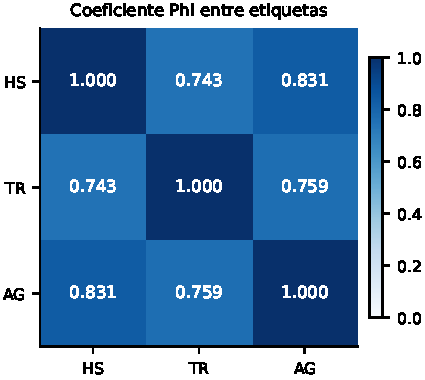
\includegraphics[width=\columnwidth]{fig_phi.pdf}
\caption{Coeficiente $\phi$ entre las tres etiquetas en entrenamiento. Los
valores altos confirman la estructura jerárquica que motiva la regla
$TR=1 \Rightarrow HS=1$.}
\label{fig:phi}
\end{figure}

\subsection{Textometría, ruido y near-duplicados}

Los textos son cortos: la longitud media es de 104.3 caracteres (mediana 91,
máximo 306) y 17.1 palabras (mediana 15). La distribución es asimétrica a la
derecha, con una cola de tuits largos que concentra una parte importante del
error, como se verá en la Sección~\ref{sec:discusion}. El corpus está
normalizado a ASCII: se pierden tildes y eñes, y con ellas parte de la señal
morfológica del español. Esa pérdida es una razón adicional para usar
n-gramas de caracteres, que reconstruyen prefijos, sufijos y variantes
ortográficas sin depender de un diccionario \cite{cavnar1994ngram,mcnamee2004character}.

La búsqueda de near-duplicados sobre la unión de entrenamiento y prueba
(2\,885 textos) encontró cuatro grupos con más de un miembro, un grupo mayor
de seis textos y 17 textos implicados. No es una duplicación masiva, pero
basta para inflar una validación ingenua. Además, se extrajo el pseudo-autor
de cada texto (la primera mención \texttt{@usuario}) y se fusionaron ambos
criterios con una estructura union-find: el entrenamiento queda en 1\,645
grupos, 86 filas menos que la partición por filas. Esa fusión es la unidad de
partición de toda la validación (Sección~\ref{sec:metodologia}). Como control
de fuga por orden, se contrastó la asociación entre el identificador y las
etiquetas: las correlaciones de Spearman fueron $+0.0166$ ($p=0.490$),
$-0.0019$ ($p=0.938$) y $-0.0070$ ($p=0.772$) para HS, TR y AG, y la prueba
$\chi^2$ del identificador agrupado en deciles contra HS dio $\chi^2(9)=12.20$, $p=0.202$. No hay evidencia de que el orden de los identificadores filtre
la etiqueta.

\subsection{Hallazgos que guiaron el modelado}

El análisis exploratorio dejó cinco decisiones estructurales. (i) El
desbalanceo moderado y distinto por etiqueta justifica pesos de clase
balanceados y umbrales desacoplados \cite{japkowicz2002class,lipton2014thresholding}.
(ii) La jerarquía HatEval justifica la regla ascendente. (iii) Los textos
cortos y ruidosos justifican una representación subléxica multiescala.
(iv) Los near-duplicados y los pseudo-autores justifican la validación
agrupada. (v) La ausencia de asociación entre identificador y etiqueta
descarta una fuga por orden. La Figura~\ref{fig:eda} resume los perfiles y
la distribución de longitudes.

\begin{figure*}[t]
\centering
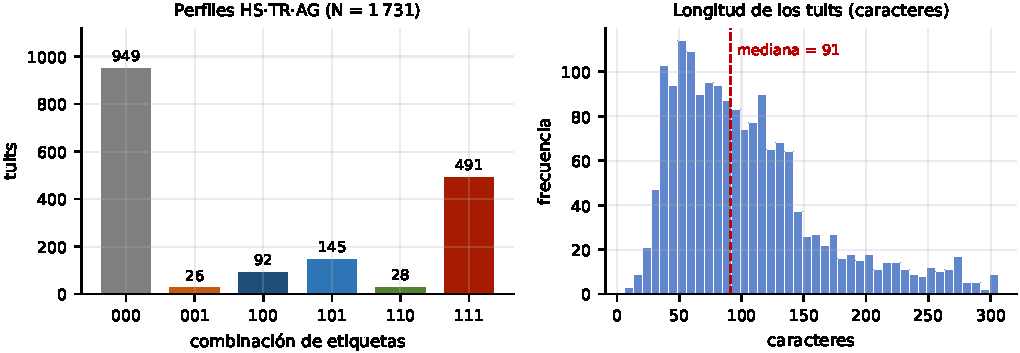
\includegraphics[width=\textwidth]{fig_eda.pdf}
\caption{Análisis exploratorio. Izquierda: perfiles HS$\cdot$TR$\cdot$AG; la
mayoría del corpus es limpio y el perfil 111 es el segundo más frecuente.
Derecha: distribución de longitudes; la mediana es 91 caracteres y la cola
larga concentra los casos más difíciles.}
\label{fig:eda}
\end{figure*}

Una tensión adicional, que no se resuelve con datos, es la definición de TR.
La competencia marca «discurso dirigido contra una persona o grupo»; HatEval
distingue entre objetivo individual y genérico, y exige que el mensaje esté dirigido a uno de ellos
\cite{basile2019hateval}. Varios errores residuales de TR son, en realidad,
desacuerdos de anotación entre esas dos lecturas. Decidimos no modificar las
etiquetas oficiales y modelar la definición de la competencia; la discrepancia
queda documentada como parte del análisis de error.
\section{Metodología}
\label{sec:metodologia}

\subsection{Marco metodológico: CRISP-DM}
\label{subsec:crispdm}

El proyecto se condujo con \emph{CRISP-DM} (\emph{Cross Industry Standard
Process for Data Mining}) como metodología principal \cite{wirth2000crisp}.
Las seis fases del ciclo se ejecutaron de forma iterativa: el proyecto
registró 134 ciclos experimentales y varias veces una fase posterior devolvió
el trabajo a una anterior. El caso más claro fue el hallazgo de la fuga por
pseudo-autores: apareció al auditar la validación y obligó a rehacer la
preparación de los datos (fusión de grupos) antes de continuar con el
modelado. La Tabla~\ref{tab:crispdm} resume el mapeo entre las fases, el
trabajo realizado y la evidencia que lo respalda.

\begin{table*}[t]
\centering
\caption{Las seis fases de CRISP-DM, el trabajo realizado y la evidencia
principal. El ciclo se recorrió varias veces; la tabla resume la ejecución
completa.}
\label{tab:crispdm}
\small
\begin{tabularx}{\textwidth}{@{}>{\raggedright\arraybackslash}p{2.1cm}X>{\raggedright\arraybackslash}p{3.1cm}@{}}
\toprule
Fase & Qué se hizo & Evidencia principal \\
\midrule
Comprensión del negocio & Se definió la tarea multietiqueta (HS, TR, AG), se registraron las reglas (sin transformers, sin etiquetas del test), se identificó la métrica con la sonda E00 (LB 0.51494) y se fijaron los criterios de éxito. & Sección I; \path{docs/competition_rules.md}; decisión D-009. \\
Comprensión de los datos & Se perfilaron 1\,731 tuits: prevalencias, perfiles conjuntos, longitudes, $\phi$, near-duplicados, pseudo-autores, asociación identificador--etiqueta y ambigüedad semántica de TR. & Sección III; \texttt{reports/eda/}; cuaderno, sección 2. \\
Preparación de los datos & Se fusionaron near-duplicados y pseudo-autores en grupos, se congelaron las particiones, se construyó V2\_triple y se verificó la ausencia de fuga en cada pliegue. & Sección IV; \path{features/}; decisiones D-004 y D-015. \\
Modelado & 134 ciclos experimentales: preprocesamiento, representación, modelos lineales, umbrales, ensembles, aprendizaje profundo desde cero, staging y pares compensados. & Secciones~\ref{sec:resultados} y~\ref{sec:arquitectura}; \texttt{experiments.csv}; \texttt{reports/}. \\
Evaluación & CCV agrupada en dos particiones, bootstrap, McNemar, análisis de error por rebanadas, holdout congelado y sondas del leaderboard. & Sección~\ref{sec:discusion}; \path{informe/datos/estadisticas.json}. \\
Despliegue & Reentrenamiento sobre el 100\,\% de \emph{train}, staging, envío, verificación SHA e idempotencia; publicación del cuaderno y de los artefactos. & Sección~\ref{sec:reproducibilidad}; \texttt{submissions/}; cuaderno. \\
\bottomrule
\end{tabularx}
\end{table*}

La gobernanza experimental complementó el ciclo. Cada experimento tuvo un
script propio y nuevo (una variación no edita el script anterior), un
pre-registro con pregunta, hipótesis y criterio de adopción, y una fila en
\texttt{experiments.csv}. La regla de adopción era exigente: una mejora local
debía superar $+0.005$ y sostenerse en las dos particiones; un candidato con
sonda debía mejorar además el leaderboard, y una mejora solo local no bastaba
(P109 es el contraejemplo). Cada corrida importante re-ejecutaba los
controles de determinismo (V03 exacto y P110 a $10^{-6}$) y el test nunca se
usó para entrenar ni para ajustar el modelo base. Esta disciplina explica por
qué el informe conserva los resultados negativos con el mismo detalle que los
positivos: son parte de la evidencia.

\subsection{Protocolo de validación agrupada}

La unidad de partición no es la fila sino el \emph{grupo fusionado}: la unión
de near-duplicados (similitud coseno de n-gramas de caracteres $\ge 0.85$) y
pseudo-autores (primera mención \texttt{@usuario}). Sobre los 1\,731 tuits se
construyen 1\,645 grupos. Con ellos se separa un desarrollo de 1\,483 filas y
un holdout congelado de 248 mediante \texttt{StratifiedGroupKFold} de siete
pliegues (semilla 42), estratificando por la combinación HS$\cdot$TR$\cdot$AG.
El desarrollo se evalúa con dos particiones de cinco pliegues: la canónica
(semilla 42) y la partición 47 (semilla 43), que actúa como réplica
independiente. Todas las métricas locales de este artículo son
\emph{out-of-fold} (OOF) sobre las 1\,483 filas de desarrollo. La línea base
del proyecto, V03, es la unión TF-IDF \texttt{word(1,2)}+\texttt{char\_wb(3,5)}
con regresión logística \textsc{liblinear} ($C=2.0$), umbrales 0.44/0.51/0.46 y
sin regla ascendente; su $F_1$ OOF es 0.777211 y su LB 0.78306. El holdout de
248 filas se reservó como guarda congelada y no se usó para las decisiones de
la serie final; por eso las cifras que se reportan son OOF sobre desarrollo.

El protocolo impone tres controles. Primero, los vectorizadores se ajustan
solo con el pliegue de entrenamiento y se aplican al de validación; el test
nunca participa. Segundo, se verifica en cada pliegue que ningún grupo
fusionado cruce la frontera entrenamiento/validación. Tercero, cada corrida
re-ejecuta dos controles de determinismo: la reconstrucción de la línea base
V03 debe coincidir exactamente (diferencia 0.0) y la de P110 dentro de
$10^{-6}$. Estos controles detectan deriva de entorno antes de comparar
candidatos \cite{kohavi1995study,kaufman2012leakage}.

\subsection{Representación subléxica multiescala}

La representación campeona, que llamamos V2\_triple, concatena tres bloques
TF-IDF \cite{joachims1998text}: palabras con unigramas y bigramas
(\texttt{word(1,2)}), n-gramas de caracteres con límites de palabra
(\texttt{char\_wb(3,5)}) y n-gramas de caracteres libres
(\texttt{char(1,6)}). Para cada bloque, el peso de un término $t$ en un
documento $d$ es
\begin{equation}
w_{t,d} = \bigl(1+\log \mathrm{tf}_{t,d}\bigr)
\left(\log\frac{1+N}{1+\mathrm{df}_t}+1\right),
\label{eq:tfidf}
\end{equation}
donde $\mathrm{tf}_{t,d}$ es la frecuencia del término en el documento (con
$w_{t,d}=0$ si el término no aparece), seguido de normalización $L_2$; se usa \texttt{min\_df}=2 y
\texttt{sublinear\_tf}=True. La unión produce 86\,275 características sobre el
corpus completo. El bloque de palabras aporta la señal semántica; los bloques
de caracteres aportan robustez frente a errores ortográficos, alargamientos
vocálicos, elisiones y jerga, que son precisamente los fenómenos que un
vocabulario de palabras no puede representar \cite{cavnar1994ngram,mcnamee2004character}.

\subsection{Modelos, ensamble y calibración}

Para cada etiqueta se ajusta una regresión logística con pesos de clase
balanceados,
\begin{equation}
p_j(x)=\sigma\bigl(\beta_{j0}+\beta_j^{\top}x\bigr), \qquad
\sigma(z)=\frac{1}{1+e^{-z}},
\label{eq:logit}
\end{equation}
con regularización $C$ adaptada por etiqueta (2.0 para HS, 1.8 para TR y 1.5
para AG). El solver es \textsc{liblinear} \cite{fan2008liblinear}. Sobre la
misma matriz se ajustan dos modelos adicionales: un \texttt{SGDClassifier}
con pérdida logarítmica y $\alpha=5\times10^{-6}$ \cite{bottou2010large}, y
una regresión logística SAGA con penalización ElasticNet
($\ell_1$-ratio 0.05) \cite{defazio2014saga,zou2005regularization}. El
ensamble, que llamamos Tri-Optimizer, combina las probabilidades
\begin{equation}
p = 0.80\,p^{\mathrm{LR}} + 0.05\,p^{\mathrm{SGD}} + 0.15\,p^{\mathrm{SAGA}},
\label{eq:ensemble}
\end{equation}
y las calibra con un escalado de temperatura en el espacio log-odds
\cite{guo2017calibration}:
\begin{equation}
\tilde p_j = \sigma\!\left(\frac{\operatorname{logit}(p_j)}{T}\right),
\qquad T=1.04.
\label{eq:temperatura}
\end{equation}
La temperatura se fijó en la fase de desarrollo y se congeló; no se ajustó
con el test. La combinación de tres optimizadores con sesgos inductivos
distintos busca reducir la varianza sin renunciar a la interpretabilidad de
un modelo lineal.

\subsection{Decisión: umbrales, regla ontológica y pares compensados}

La binarización usa un umbral por etiqueta,
\begin{equation}
\hat y_j = \mathbb{1}\left[\tilde p_j \ge \tau_j\right], \qquad
\tau = (0.44,\;0.51,\;0.46),
\label{eq:umbral}
\end{equation}
y después aplica la regla ascendente de HatEval: si $TR=1$ y $HS=0$, se
fuerza $HS=1$. Los umbrales se fijaron en la fase de calibración (desarrollo y
leaderboard público) con un criterio de $F_1$ por columna
\cite{lipton2014thresholding,nan2012optimizing} y se congelaron antes de la
serie final; no se usaron etiquetas del test. La métrica oficial es
\begin{equation}
\begin{split}
M &= \frac{1}{3}\sum_{j\in\{\mathrm{HS},\mathrm{TR},\mathrm{AG}\}} F_1^{(j)},\\
F_1^{(j)} &= \frac{2TP_j}{2TP_j+FP_j+FN_j}.
\end{split}
\label{eq:f1}
\end{equation}

Sobre esa base actúa la capa de decisión de la serie P120--P133. Su
componente principal son los \emph{pares compensados}: un lote de reglas
léxicas que rescata verdaderos positivos y suprime falsos positivos, con la
restricción de que el número de celdas activadas y desactivadas sea el mismo
en cada columna. La propiedad central se resume en la siguiente proposición.

\begin{proposicion}[Economía del par compensado]
\label{prop:par}
Sea una columna con $TP$, $FP$ y $FN$ celdas, y sea $D=2TP+FP+FN$. Si un
lote compensado rescata $a$ verdaderos positivos ($FN\to TP$) y suprime $a$
falsos positivos ($FP\to TN$) en esa columna, entonces
\begin{equation}
F_1' = F_1 + \frac{2a}{D} = F_1 + a\,\frac{F_1}{TP}.
\label{eq:par}
\end{equation}
El número de positivos de la columna no cambia.
\end{proposicion}

\begin{proof}
Tras el lote, $TP'=TP+a$, $FP'=FP-a$ y $FN'=FN-a$, de modo que
$D'=2(TP+a)+(FP-a)+(FN-a)=D$. Entonces
$F_1'=2(TP+a)/D=F_1+2a/D$. Como $F_1=2TP/D$, se tiene $2/D=F_1/TP$, y
sustituyendo se obtiene \eqref{eq:par}.
\end{proof}

La proposición explica por qué la ganancia de un par es predecible y por qué
la columna minoritaria es la más sensible: a igualdad de $a$, el incremento
$F_1/TP$ es mayor cuando $TP$ es pequeño, que es el caso de TR. También
describe el escenario óptimo: los $a$ rescates corresponden a verdaderos
positivos del conjunto oculto y las $a$ supresiones a falsos positivos reales.
Si una intervención rescata un caso que los anotadores consideraron negativo o
suprime un positivo genuino, la compensación se rompe y la ganancia se anula o
se vuelve negativa; P129 es la evidencia empírica de ese caso. En la implementación, el desplazamiento se aplica en log-odds
($\pm 2.0$ o $\pm 2.05$) para no saturar la probabilidad; la versión P129,
con un desplazamiento forzado de $+4.0$, ilustra el costo de romper la
compensación (Sección~\ref{sec:resultados}).

El lote P133, el campeón, contiene nueve pares: cuatro en HS, dos en TR y
tres en AG. Las firmas léxicas se diseñaron para tener cero coincidencias en
entrenamiento y una coincidencia exacta en test; por construcción, no
cambian la métrica OOF. La capa mantiene el \emph{ancla de prevalencia}
$\mathbf{n}=(514,330,421)$, es decir, 1\,265 positivos (36.54\,\%). El ancla no
es una estimación poblacional independiente: es la tasa de positivos que
maximizó el leaderboard en la fase de calibración y se usa como restricción
de invariancia. Esa distinción se discute en la Sección~\ref{sec:discusion}.

\subsection{Análisis estadístico}

Las comparaciones entre modelos usan bootstrap agrupado con 2\,000 réplicas y
semilla 20260925: se remuestrean grupos completos, no filas, para conservar
la dependencia \cite{efron1979bootstrap}. Los intervalos son percentiles al
95\,\%. Para los aciertos pareados se aplica la prueba exacta de McNemar
sobre las celdas discordantes \cite{mcnemar1947note,dietterich1998approximate}.
Las prevalencias se acompañan de intervalos de Wilson
\cite{wilson1927probable}; la asociación entre etiquetas se mide con $\phi$ y
$\chi^2$. La sensibilidad al umbral se resume en curvas $F_1$--$\tau$ por
etiqueta, y el error se desglosa por franjas de longitud (terciles en 70 y
118 caracteres). No se aplican correcciones por comparaciones múltiples
porque el número de hipótesis confirmatorias es pequeño y están
pre-registradas; los valores $p$ se reportan como evidencia, no como un
cribado masivo \cite{demsar2006statistical}.

La Tabla~\ref{tab:decisiones} sintetiza las decisiones de diseño y la
evidencia que las sostiene.

\begin{table*}[t]
\centering
\caption{Decisiones de diseño, alternativas consideradas y evidencia que las
sostiene. Las cifras locales son OOF sobre 1\,483 filas; las del leaderboard
son el registro público de Kaggle.}
\label{tab:decisiones}
\small
\begin{tabularx}{\textwidth}{@{}>{\raggedright\arraybackslash}p{2.0cm}>{\raggedright\arraybackslash}p{2.6cm}X>{\raggedright\arraybackslash}p{2.3cm}@{}}
\toprule
Decisión & Alternativa & Evidencia & Consecuencia \\
\midrule
Tres clasificadores binarios & Una clase con seis combinaciones & 0 casos $TR=1,HS=0$; 26 casos $AG=1,HS=0$; $\phi$ alto & Se adopta, con regla ascendente \\
Representación V2\_triple & Solo palabras o unión de dos bloques & $+0.00516$ local y $+0.00549$ LB frente a V03 & Se adopta \\
Tri-Optimizer & Mezcla 95/5 LR+SGD (P110) & $+0.00222$ local y $+0.00090$ LB; 4/5 y 3/5 pliegues & Se adopta \\
Umbrales por etiqueta & Umbral único 0.5 & $+0.00313$ LB en la línea base & Se congelan 0.44/0.51/0.46 \\
Validación agrupada & Validación por filas & 1\,645 grupos (86 filas menos); 0 fugas verificadas & Se adopta en todo el proyecto \\
Pares compensados & Staging masivo o unilateral & P128 $+0.00999$; P129 $-0.00438$ & Lotes pequeños, contables y verificados en LB \\
\bottomrule
\end{tabularx}
\end{table*}

La Figura~\ref{fig:arquitectura} resume la arquitectura del sistema.

\begin{figure*}[t]
\centering
\begin{tikzpicture}[
  node distance=2.6mm,
  stage/.style={draw, rounded corners, align=center, font=\footnotesize,
    inner sep=3pt, minimum height=9mm, text width=1.7cm},
  note/.style={draw=none, align=center, font=\scriptsize, text=black!65},
  arrow/.style={-{Latex[length=1.6mm]}, line width=0.5pt}
]
\node[stage] (corpus) {Corpus\\1\,731 / 1\,154};
\node[stage, right=of corpus] (tfidf) {TF-IDF\\V2\_triple\\86\,275};
\node[stage, right=of tfidf] (model) {Tri-Optimizer\\80/5/15\\$T=1.04$};
\node[stage, right=of model] (dec) {Umbrales\\0.44/0.51/0.46\\+ HatEval};
\node[stage, right=of dec] (pairs) {Pares\\compensados\\ancla};
\node[stage, right=of pairs] (out) {Envío\\+ SHA256};
\draw[arrow] (corpus) -- (tfidf);
\draw[arrow] (tfidf) -- (model);
\draw[arrow] (model) -- (dec);
\draw[arrow] (dec) -- (pairs);
\draw[arrow] (pairs) -- (out);
\node[note, below=3mm of tfidf] (val) {validación agrupada\\OOF (1\,483)};
\node[note, below=3mm of pairs] (lb) {sondas LB\\47 envíos};
\draw[arrow, dashed] (val) -- (tfidf);
\draw[arrow, dashed] (lb) -- (pairs);
\end{tikzpicture}
\caption{Arquitectura del sistema. La validación agrupada gobierna la
representación y el modelo; las sondas del leaderboard gobiernan únicamente
la capa de pares compensados. La separación es deliberada: son dos fuentes de
evidencia distintas.}
\label{fig:arquitectura}
\end{figure*}

\section{Experimentación y resultados}
\label{sec:resultados}

\subsection{La serie final}

La serie final comprende veintiséis candidatos, de los cuales veinticinco se
evaluaron en el leaderboard público; P123 quedó listo pero no se envió. En
total, el proyecto realizó 47 envíos de modelos al leaderboard (más una
sonda de plantilla); 25 corresponden a esta
serie. La Tabla~\ref{tab:serie} reúne todos los experimentos con su métrica local en
las dos particiones congeladas, su $F_1$ público y la decisión registrada.
Las cifras locales se re-ejecutaron desde las probabilidades OOF; las del
leaderboard son el registro externo de Kaggle y no son recomputables.

\begin{table*}[t]
\centering
\caption{La serie final (P108--P133, sin P123). CCV es la $F_1$ media
columnar out-of-fold sobre las 1\,483 filas de desarrollo; LB es el $F_1$
público de Kaggle. P123 no se envió y se omite. El registro interno del
leaderboard guarda la media de las dos particiones; aquí se reportan por
separado.}
\label{tab:serie}
\scriptsize
\setlength{\tabcolsep}{4.5pt}
\begin{tabular*}{\textwidth}{@{\extracolsep{\fill}}lrrrl@{}}
\toprule
Exp. & CCV canónica & CCV partición 47 & LB público & Decisión \\
\midrule
P108 & 0.782372 & 0.781185 & 0.78855 & Adoptado \\
P109 & 0.792215 & 0.789294 & 0.77447 & Descartado (min\_df=5) \\
P110 & 0.784998 & 0.784318 & 0.78967 & Mejor LB \\
P111 & 0.786912 & 0.785868 & 0.78951 & Descartado \\
P112 & 0.780834 & 0.781824 & 0.78652 & Descartado \\
P113 & 0.787241 & 0.785049 & 0.78664 & Descartado \\
P114 & 0.787218 & 0.785673 & 0.79057 & Mejor LB \\
P115 & 0.788431 & 0.787190 & 0.78825 & Descartado \\
P116 & 0.786348 & 0.788892 & 0.78975 & Descartado \\
P117 & 0.787967 & 0.787259 & 0.78885 & Descartado \\
P118 & 0.787881 & 0.786026 & 0.78930 & Descartado \\
P119 & 0.785897 & 0.784121 & 0.78860 & Descartado \\
P120 & 0.787582 & 0.785673 & 0.79035 & Descartado \\
P121 & 0.787582 & 0.785673 & 0.79095 & Mejor LB \\
P122 & 0.787582 & 0.786034 & 0.79095 & Empate técnico \\
P124 & 0.787127 & 0.785810 & 0.79095 & Neutral \\
P125 & 0.787127 & 0.785810 & 0.79337 & Mejor LB \\
P126 & 0.787127 & 0.785810 & 0.79375 & Mejor LB \\
P127 & 0.787582 & 0.786034 & 0.79517 & Mejor LB \\
P128 & 0.787582 & 0.786034 & 0.80516 & Mejor LB histórico \\
P129 & 0.787582 & 0.786034 & 0.80078 & Descartado (offset 4.0) \\
P130 & 0.787582 & 0.786034 & 0.80516 & Empate técnico \\
P131 & 0.787582 & 0.786034 & 0.80872 & Mejor LB \\
P132 & 0.787582 & 0.786034 & 0.81279 & Mejor LB ($>0.81$) \\
P133 & 0.787582 & 0.786034 & 0.81447 & Envío final \\
\midrule
\multicolumn{5}{l}{\scriptsize * P123 (CCV 0.788584 / 0.786034) quedó listo en desarrollo local y no se envió a Kaggle.} \\
\bottomrule
\end{tabular*}
\end{table*}

\subsection{Qué funcionó}

La primera ganancia vino de la representación. P108 sustituyó la unión de dos
bloques de V03 por V2\_triple y pasó de 0.777211 a 0.782372 en la partición
canónica ($+0.005160$) y de 0.78306 a 0.78855 en el leaderboard
($+0.00549$). La mejora se replicó en la partición 47 ($+0.005553$), de modo
que no fue una fluctuación de una sola partición.

La segunda ganancia vino del ensamble. P110 mezcló 95\,\% de la regresión
logística con 5\,\% de SGD y subió a 0.784998 local y 0.78967 en el
leaderboard. P114 añadió SAGA con ElasticNet, calibró la temperatura en 1.04
y alcanzó 0.787218 local ($+0.002220$ sobre P110) y 0.79057 en el
leaderboard. La mejora se observó en cuatro de los cinco pliegues de la
partición canónica y en tres de los cinco de la partición 47. El
Tri-Optimizer se convirtió en la base de todo lo que siguió: a partir de
P114 el proyecto dejó de cambiar la representación y los modelos, y concentró
el esfuerzo en la decisión.

La tercera ganancia vino de las leyes de decisión. P121 fijó el staging
asimétrico y el ancla de prevalencia: 0.79095 en el leaderboard. El salto
grande llegó con los pares compensados. P125 sumó el primer par doble
($+0.00242$), P126 el segundo ($+0.00038$), P127 el tercero ($+0.00142$) y
P128 el lote de quince pares que cruzó la barrera de 0.80
($+0.00999$). Después de P128, P131 recuperó la fila 114 y sumó siete pares
($+0.00356$, primer lugar), P132 sumó otros siete ($+0.00407$, primer
registro por encima de 0.81) y P133 sumó nueve ($+0.00168$, 0.81447). La
Figura~\ref{fig:escalera} muestra la divergencia entre la métrica local y el
leaderboard: las variantes P127--P133 comparten exactamente la misma CCV
porque sus reglas no disparan en entrenamiento; P124--P126, con la escalera
histórica, quedan en 0.787127. Solo el leaderboard las distingue.

\begin{figure*}[t]
\centering
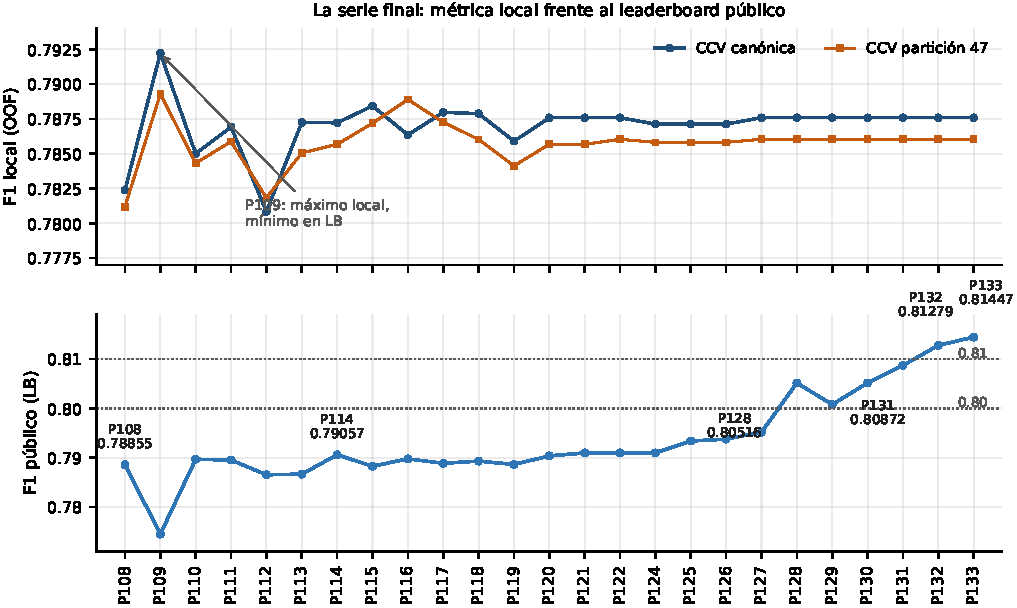
\includegraphics[width=\textwidth]{fig_escalera.pdf}
\caption{La serie final. Arriba: $F_1$ out-of-fold en las dos particiones
congeladas. Abajo: $F_1$ público de Kaggle. P109 es el caso paradigmático de
divergencia: la mejor métrica local de la serie (0.792215) produjo el peor
resultado público (0.77447). Las variantes P127--P133 comparten la misma
métrica local porque sus reglas léxicas no aparecen en entrenamiento;
P124--P126 usan la escalera histórica y quedan en 0.787127.}
\label{fig:escalera}
\end{figure*}

\subsection{Qué no funcionó}

El fracaso más instructivo fue P109. La poda por frecuencia
(\texttt{min\_df}=5) y la recalibración de umbrales produjeron la mejor
métrica local de toda la serie (0.792215 canónica, 0.789294 en la partición
47), pero el leaderboard cayó a 0.77447, por debajo de V03. La explicación es
mecánica: la poda elimina términos raros que sostienen la señal en un corpus
pequeño; la validación local, al compartir el mismo vocabulario podado,
sobreestima la transferencia. P109 se rechazó y se convirtió en la evidencia
de que la decisión debía mirar el leaderboard, no solo la CCV.

La familia de ensambles alternativos tampoco superó a P114. P111 (mezcla
95/5 con $C$ adaptada) quedó en 0.78951; P112 (bagging de diez pliegues) en
0.78652; P113 (tri-blend con pérdida de margen) en 0.78664. P115 (gating
ontológico dual) mejoró la métrica local hasta 0.788431 pero cayó a 0.78825
en el leaderboard: los rescates sobrepredijeron positivos en el test ciego.
P116--P119 exploraron \texttt{max\_df}=0.90, NBSVM, BM25 con SVD y un canal
de mención; ninguno superó a P114 en el leaderboard (0.78975, 0.78885,
0.78930 y 0.78860). P120, con las tres leyes de staging completas, quedó en
0.79035; P122 y P124 empataron con P121 en 0.79095.

P129 es el contraejemplo de la Proposición~\ref{prop:par}. Once pares con un
desplazamiento forzado de $+4.0$ en log-odds saturaron la probabilidad
($\sigma(z+4)>0.98$), rompieron la escala del ranking e hicieron perder tres
predicciones positivas de TR que el envío anterior conservaba. El resultado fue
0.80078, una
caída de 0.00438 frente a P128. P130 intentó suprimir la fila 114 (una cita
irónica de \emph{Dr. House}) y empató exactamente con P128 en 0.80516: la
supresión anuló el beneficio de los rescates. La lección fue doble: las
frases de ficción no se suprimen sin evidencia inequívoca y los lotes deben
ser pequeños, contables y con desplazamientos moderados. La
Tabla~\ref{tab:rechazos} detalla, para cada candidato descartado, la
hipótesis que lo motivó y la razón concreta del rechazo.

\begin{table*}[t]
\centering
\caption{Por qué se rechazaron los candidatos de la serie final que no
llegaron a campeones. La primera cifra de cada resultado es la CCV canónica y
la segunda el LB público.}
\label{tab:rechazos}
\scriptsize
\begin{tabularx}{\textwidth}{@{}>{\raggedright\arraybackslash}p{1.5cm}>{\raggedright\arraybackslash}p{4.3cm}>{\raggedright\arraybackslash}p{2.5cm}X@{}}
\toprule
Exp. & Hipótesis y motivación & Resultado (CCV / LB) & Motivo del rechazo \\
\midrule
P109 & La poda por frecuencia (\texttt{min\_df}=5) reduce ruido; los umbrales se recalibran. & 0.792215 / 0.77447 & El vocabulario podado no transfiere: la validación comparte la poda y el test no. \\
P111--P113 & Mezclas 95/5 con $C$ adaptada, bagging de diez pliegues y pérdida de margen. & 0.7869 / 0.78951; 0.7808 / 0.78652; 0.7872 / 0.78664 & Ninguna supera a P114 (0.79057) en el leaderboard. \\
P115 & Gating ontológico dual: rescates de HS y TR guiados por la estructura de etiquetas. & 0.788431 / 0.78825 & Los rescates sobrepredicen positivos en el test ciego. \\
P116--P119 & \texttt{max\_df}=0.90, subespacio NBSVM, BM25 con SVD y canal de mención. & 0.7863--0.7880 / 0.78860--0.78975 & Ninguno supera a P114; la mejora local no se replica. \\
P120 & Las tres leyes de staging conjuntas. & 0.787582 / 0.79035 & La ley de TR no transfiere; P121 la apaga y gana $+0.00060$. \\
P122 y P124 & Variantes de covarianza y de rescate público. & 0.787582 / 0.79095 & Empatan con P121: sin ganancia medible. \\
P129 & Once pares con un desplazamiento forzado de $+4.0$ en log-odds. & 0.787582 / 0.80078 & Satura la probabilidad y rompe el ranking: $-0.00438$ frente a P128. \\
P130 & Suprimir la fila 114 (cita irónica de una serie de televisión). & 0.787582 / 0.80516 & Empate exacto con P128: la supresión anula el beneficio de los rescates. \\
\bottomrule
\end{tabularx}
\end{table*}


Las fases anteriores a P108 dejaron un catálogo de resultados negativos que
conviene registrar con el mismo detalle que los positivos. La
Tabla~\ref{tab:familias} los resume: cada familia partió de una hipótesis
concreta, se evaluó con el protocolo agrupado y se cerró cuando no superó la
barrera de adopción. El patrón es consistente: de más de cincuenta
configuraciones evaluadas, solo la representación de n-gramas con regresión
logística regularizada y umbrales por etiqueta se adoptó como modelo final.
La fase v2 exploró veinticuatro líneas adicionales (meta-modelos, calibración,
especialistas por rebanada, codificación de menciones); su mejor candidato
mejoró $+0.0081$ en desarrollo y $+0.0180$ en el holdout congelado, pero no
transfirió al leaderboard (0.78163 frente a 0.78306 de V03).
El resultado recurrente fue el mismo: el residuo no es información ausente
que el modelo no sepa extraer, sino una frontera de anotación. En la región
de insulto interpersonal con mención inicial y sin referencia colectiva,
40.49\,\% de los textos está etiquetado como limpio; ningún modelo de texto
puede recuperar esa distinción sin la etiqueta.

Las fases previas a P108 exploraron también representaciones densas entrenadas
desde cero, bajo estricto cumplimiento de las reglas. En las fases v5, v21,
P98 y P99 se compiló y auditó un corpus externo en español de 29.7 millones de
tokens (Wikipedia-es 18.0\,M, mC4-es 7.5\,M y Twitter COVID-es 4.5\,M), con
licencias abiertas y cero solapamiento con el corpus de la competencia. Sobre
ese corpus se entrenaron modelos FastText de 200 dimensiones
\cite{bojanowski2017enriching} y un modelo de lenguaje recurrente
bidireccional (LTR y RTL, cuatro épocas cada uno; perplejidad de validación
91.7--94.8). El resultado fue claro: los embeddings por sí solos alcanzaron
$F_1 \approx 0.652$ OOF, muy por debajo del 0.777 de TF-IDF; su concatenación
con la matriz dispersa aportó $+0.0046$ local, pero el IC95 cruzaba el cero
($[-0.003, +0.012]$) y no transfirió al leaderboard. En textos cortos
(mediana 91 caracteres) con ruido léxico y alargamientos vocálicos, el
promediado de vectores diluye la señal; los n-gramas de caracteres conservan
directamente los morfemas y las raíces de toxicidad.

\begin{table*}[t]
\centering
\caption{Familias experimentales anteriores a P108: hipótesis, resultado y
decisión. El patrón común fue que las mejoras locales no transfirieron al
leaderboard o no superaron la barrera de adopción de $+0.005$.}
\label{tab:familias}
\scriptsize
\begin{tabularx}{\textwidth}{@{}>{\raggedright\arraybackslash}p{2.5cm}X>{\raggedright\arraybackslash}p{3.6cm}>{\raggedright\arraybackslash}p{2.6cm}@{}}
\toprule
Familia & Hipótesis y motivación & Resultado & Decisión \\
\midrule
Sonda de métrica y baselines & Identificar la métrica oficial y fijar una referencia reproducible. & Todo-uno: LB 0.51494; B1 (TF-IDF de palabras + LR): OOF 0.7587 y LB 0.75677; B5 denso: OOF 0.6607. & Métrica confirmada (media columnar); B1 como referencia. \\
Preprocesamiento (10 variantes) & Normalizar URLs, lematizar, preservar mayúsculas, quitar \emph{stopwords} o puntuación. & La mejor (URLs como token) sumó $+0.0035$; lematización $-0.0162$; mayúsculas $-0.0229$; \emph{stopwords} $-0.0025$. & Descartadas: ninguna superó la barrera de $+0.005$. \\
Representación y modelos & La unión de palabras y caracteres aporta; un modelo lineal regularizado compite. & Unión: $+0.0278$ con 5/5 pliegues; ComplementNB 0.6888; LinearSVC 0.7849; LR con $C=2.0$ 0.7927. & Adoptadas la unión y la LR; el resto descartado. \\
Post-proceso jerárquico & Explotar $HS=0 \Rightarrow TR=0, AG=0$ para eliminar positivos incoherentes. & $-0.0056$ sobre el modelo que lo origina. & Descartado. \\
Rasgos densos y lexicones & Añadir deshumanización, registro bromista y objetivo individual o colectivo. & Entre $-0.0091$ y $-0.0316$; con las densas a cero el pipeline reproduce MOD-03b exacto. & Descartadas; el control descarta un artefacto de implementación. \\
Ensembles & Combinar modelos diversos para reducir varianza. & Máximo $+0.0023$ anidado; el envío v04 cayó a LB 0.77510. & Descartados. \\
Optuna y robustez & Optimizar hiperparámetros y reducir capacidad para transferir mejor. & Optuna: OOF 0.8039 y LB 0.77602; $C=1.0$: LB 0.77227; \texttt{min\_df}=5: LB 0.77034. & Descartados: el mejor OOF fue el peor LB. \\
Aprendizaje profundo desde cero & Requisito metodológico: MLP, CharCNN y BiLSTM sin embeddings preentrenados. & MLP 0.7949 OOF; CharCNN 0.7410; BiLSTM 0.7364; sin sonda de LB. & No adoptado: no superó la regla de $+0.005$ con evidencia externa. \\
Validación por pseudo-autor & Comprobar que los pliegues no compartan usuarios. & 17/17 autores con $\ge 3$ tuits cruzaban pliegues; al fusionar grupos, OOF $0.7927 \to 0.7838$ y el gap local-LB pasó de $-0.0128$ a $-0.0039$. & Adoptado como protocolo (D-015). \\
Preentrenamiento y embeddings desde cero (v5, v21, P98, P99) & Entrenar FastText (200\,d) y un modelo de lenguaje recurrente desde cero sobre un corpus externo de 29.7\,M de tokens. & Solo embeddings: OOF 0.6522--0.6530, frente a 0.7772 de TF-IDF; fusión \emph{hstack}: 0.7818--0.7829, delta local $+0.0046$ con IC95 $[-0.003, +0.012]$ que cruza el cero; sin transferencia al LB. & Descartados: el promediado continuo diluye la señal en textos cortos y ruidosos. \\
\midrule
Complejidad no lineal y optimizadores (v23--v44, P45--P107) & Probar clasificadores no lineales (SVC-RBF, Tsetlin Machine, PLS, Group DRO, NNPU, Factorization Machines). & El SVC-RBF alcanzó 0.7904 OOF con un intervalo frágil; ninguno superó de forma transferible a la regla lineal $L_2$. & Descartadas: se ratifica la parsimonia lineal. \\
\midrule
Meta-modelos y reetiquetado (v2, v4, P87--P93) & Buscar señal restante en meta-modelos de dependencia de etiquetas y en la revisión humana de anotaciones. & Mejor candidato v2: $+0.0081$ en desarrollo y $+0.0180$ en holdout, LB 0.78163; ninguna línea superó a V03. & Cerradas; el modelo final siguió siendo V03 y después P108. \\
\bottomrule
\end{tabularx}
\end{table*}


\subsection{Descomposición de la ganancia}

La Figura~\ref{fig:waterfall} descompone los 0.03141 puntos que separan a
V03 (0.78306) de P133 (0.81447). El modelo base aportó $+0.00751$ (V03 a
P114); las leyes de decisión, $+0.00038$ (P114 a P121); los pares de P128,
$+0.01421$ (P121 a P128); y los pares finos de P131--P133, $+0.00931$ (P128
a P133). La asimetría es el hallazgo central: el 76\,\% de la ganancia del
leaderboard proviene de la capa de decisión, no del modelo. Esa capa es
precisamente la que no puede validarse con la OOF, porque sus reglas se
diseñaron para textos del test.

\begin{figure}[t]
\centering
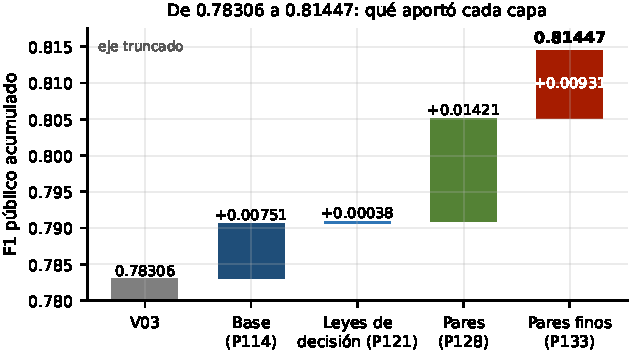
\includegraphics[width=0.92\columnwidth]{fig_waterfall.pdf}
\caption{Descomposición de la ganancia del leaderboard por capas. El eje
está truncado en 0.780 para hacer visibles las diferencias; la altura de cada
barra es la ganancia acumulada, no el valor absoluto.}
\label{fig:waterfall}
\end{figure}

\subsection{El campeón P133}

P133 es un lote de nueve pares: cuatro en HS, dos en TR y tres en AG, con
desplazamientos de $\pm2.05$ en log-odds. Los rescates activan textos con
agresiones severas contra mujeres y xenofobia explícita; las supresiones
desactivan textos de humor de animación y bromas informales que el envío
anterior marcaba como positivos y el leaderboard sugiere que eran falsos
positivos. El envío conserva el
ancla $(514,330,421)$, no presenta violaciones de la regla HatEval y tiene
una huella SHA256
\texttt{b0979a8a\ldots}. En el leaderboard público alcanzó 0.81447, con una
ventaja de $+0.00212$ sobre el segundo clasificado en el momento de la
medición. La Tabla~\ref{tab:serie} y la Figura~\ref{fig:escalera} lo sitúan
como el máximo de la serie en el leaderboard público; su métrica OOF es
idéntica a la de las variantes P127--P133, algo mayor que la de P124--P126
(0.787127) y menor que la de P109.

\section{Síntesis: la arquitectura final y su genealogía}
\label{sec:arquitectura}

\subsection{La receta final}

La arquitectura final es una tubería clásica de dos capas. La primera produce
probabilidades calibradas por etiqueta a partir de una representación
subléxica; la segunda convierte esas probabilidades en un envío multietiqueta
y aplica un lote pequeño de pares compensados. La
Figura~\ref{fig:arquitectura} muestra el flujo y la
Tabla~\ref{tab:receta} fija la configuración exacta que reconstruye el envío.

\begin{table*}[t]
\centering
\caption{Receta final del sistema P133. Cada fila es un componente que se
puede reconstruir desde los artefactos públicos; la columna de evidencia
señala el experimento o la sección que lo justifica.}
\label{tab:receta}
\scriptsize
\begin{tabularx}{\textwidth}{@{}>{\raggedright\arraybackslash}p{2.5cm}>{\raggedright\arraybackslash}X>{\raggedright\arraybackslash}p{2.9cm}@{}}
\toprule
Componente & Configuración exacta & Evidencia \\
\midrule
Corpus y particiones & 1\,731 tuits; 1\,645 grupos fusionados; desarrollo de 1\,483 filas y holdout de 248; dos particiones de cinco pliegues (semillas 42 y 43), estratificadas por HS$\cdot$TR$\cdot$AG. & Sección IV-B; cero fugas verificadas. \\
Representación & V2\_triple: \texttt{word(1,2)} + \texttt{char\_wb(3,5)} + \texttt{char(1,6)}; 86\,275 características; \texttt{min\_df}=2; \texttt{sublinear\_tf}; normalización $L_2$. & P108: $+0.00516$ local y $+0.00549$ público. \\
Modelos base & Tres clasificadores binarios por etiqueta: regresión logística \textsc{liblinear} ($C=2.0/1.8/1.5$), SGD logarítmico ($\alpha=5\times10^{-6}$) y SAGA con ElasticNet ($\ell_1$-ratio 0.05); pesos de clase balanceados. & P110 y P114; Tabla~\ref{tab:decisiones}. \\
Ensamble & $p=0.80\,p^{\mathrm{LR}}+0.05\,p^{\mathrm{SGD}}+0.15\,p^{\mathrm{SAGA}}$. & P114: $+0.00222$ local y $+0.00090$ público sobre P110. \\
Calibración & Escalado de temperatura en log-odds con $T=1.04$; se congela antes de la serie final. & P114; meseta de calibración. \\
Umbrales & $\tau=(0.44,0.51,0.46)$, fijados con el criterio de $F_1$ por columna; no se usan etiquetas del test. & V03 y P121; $+0.00313$ público. \\
Regla HatEval & Si $TR=1$ y $HS=0$, se fuerza $HS=1$; la regla se aplica después de los umbrales. & P121; cero violaciones en el envío. \\
Capa de decisión & Nueve pares compensados (cuatro HS, dos TR y tres AG), con desplazamientos de $\pm2.05$ en log-odds; ancla de prevalencia $(514,330,421)$, 1\,265 positivos (36.54\,\%). & P133: 0.81447 público; 0.787582 OOF. \\
Entrenamiento final & 100\,\% de \emph{train}; tres clasificadores por etiqueta; 1\,154 filas de test; sin etiquetas del test. & Sección~\ref{sec:reproducibilidad}; auditoría del envío. \\
Verificación & 1\,154 filas; ancla $(514,330,421)$; cero violaciones de HatEval; SHA256 \texttt{b0979a8a\ldots}; dos ejecuciones independientes. & Sección~\ref{sec:reproducibilidad}; reconstrucción bit a bit. \\
\bottomrule
\end{tabularx}
\end{table*}

La receta se puede leer en una frase: V2\_triple alimenta un Tri-Optimizer de
tres modelos lineales, calibrado a $T=1.04$, con umbrales 0.44/0.51/0.46 y la
regla ascendente de HatEval; sobre esa base, P133 aplica nueve pares
compensados y conserva el ancla. Nada de eso usa etiquetas del test: los pares
se definen por firmas léxicas con cero coincidencias en entrenamiento y se
aceptan con el leaderboard público.

\subsection{Dos capas, dos evidencias}

La distinción central del artículo es que la arquitectura tiene dos capas con
estatus epistémico distinto. La Tabla~\ref{tab:capas} lo resume. El modelo base
---representación, ensamble, calibración, umbrales y regla HatEval--- se valida
con la CCV agrupada, bootstrap y McNemar; su OOF es 0.787582 y su mejora sobre
V03 es $+0.010370$ con IC95 $[+0.003924,+0.017386]$. La capa de decisión ---los
nueve pares y el ancla--- se valida con el leaderboard; su OOF es idéntica a la
del modelo base porque las reglas no disparan en entrenamiento, y su
contribución es el 76\,\% de la ganancia pública.

\begin{table*}[t]
\centering
\caption{Las dos capas de la arquitectura final y su fuente de evidencia. La
capa base generaliza; la capa de decisión es específica del test y se valida
con sondas del leaderboard. Las cifras OOF son sobre las 1\,483 filas de
desarrollo.}
\label{tab:capas}
\scriptsize
\begin{tabularx}{\textwidth}{@{}>{\raggedright\arraybackslash}p{2.2cm}>{\raggedright\arraybackslash}X>{\raggedright\arraybackslash}p{3.3cm}>{\raggedright\arraybackslash}p{2.7cm}@{}}
\toprule
Capa & Componentes y métrica & Evidencia & Estatus \\
\midrule
Base & V2\_triple + Tri-Optimizer + $T=1.04$ + umbrales + HatEval. OOF 0.787582; P114, antes del staging, 0.787218. & CCV agrupada, bootstrap, McNemar; $+0.010370$ sobre V03 con IC95 $[+0.003924,+0.017386]$. & Generalizable; es la estimación limpia. \\
Decisión & Nueve pares compensados ($\pm2.05$) y ancla $(514,330,421)$. LB 0.81447; mismo OOF que la base. & 47 envíos al leaderboard; 25 de la serie final; deltas pareados y auditados. & Específica del test; 76\,\% de la ganancia pública. \\
\bottomrule
\end{tabularx}
\end{table*}

Esta separación explica por qué el artículo reporta dos cifras: 0.787582 es la
estimación limpia de generalización; 0.81447 es el resultado de la competencia.
Confundirlas sería el error más costoso de la narrativa. La capa de decisión no
es un modelo que hayamos entrenado con el test: es una adaptación controlada,
con pares contables, ancla de prevalencia y auditoría previa a cada envío. Aun
así, su validez externa es limitada y se discute en la
Sección~\ref{sec:discusion}.

\subsection{La ruta desde el estado del arte}

La Tabla~\ref{tab:sota} traduce cada idea del estado del arte en la decisión
experimental que la puso a prueba. La arquitectura final no se eligió por
preferencia: es el superviviente de una eliminación empírica. Cada fila tiene
una hipótesis, un experimento y un criterio de muerte; las que se adoptaron
pasaron la barrera de $+0.005$ o se sostuvieron en las dos particiones y en el
leaderboard.

\begin{table*}[t]
\centering
\caption{Del estado del arte a la decisión experimental. La tabla no repite
los 25 candidatos de la serie final; fija las ideas que estructuraron la
búsqueda y el experimento que las evaluó.}
\label{tab:sota}
\scriptsize
\begin{tabularx}{\textwidth}{@{}>{\raggedright\arraybackslash}p{4.7cm}>{\raggedright\arraybackslash}p{2.0cm}>{\raggedright\arraybackslash}X>{\raggedright\arraybackslash}p{2.1cm}@{}}
\toprule
Idea del estado del arte & Experimento & Evidencia & Decisión \\
\midrule
TF-IDF y clasificador lineal \cite{salton1988term,joachims1998text} & V03 & 0.777211 OOF; 0.78306 LB; referencia del proyecto. & Adoptado como base. \\
N-gramas de carácter para ruido ortográfico \cite{cavnar1994ngram,mcnamee2004character} & P108 & $+0.00516$ local; $+0.00549$ LB; replicado en la partición 47. & Adoptado. \\
Ensamble de optimizadores lineales \cite{breiman1996bagging,wolpert1992stacked,bottou2010large,defazio2014saga,zou2005regularization} & P110 y P114 & P110: $+0.00112$ LB; P114: $+0.00222$ local y $+0.00090$ LB sobre P110. & Adoptado (Tri-Optimizer). \\
Calibración de probabilidades \cite{platt1999probabilistic,guo2017calibration} & P114 & $T=1.04$; meseta estable; no se ajusta con el test. & Adoptado. \\
Umbrales por etiqueta \cite{lipton2014thresholding,nan2012optimizing} & V03 y P121 & $+0.00313$ LB frente al umbral único; 0.44/0.51/0.46. & Adoptado. \\
Jerarquía de etiquetas \cite{silla2011survey,basile2019hateval} & P121 & Regla $TR=1\Rightarrow HS=1$; cero violaciones. & Adoptado. \\
Pares compensados y economía de la $F_1$ \cite{flach2003geometry,saito2015precision} & P124--P133 & P128: 0.80516; P133: 0.81447; P129: $-0.00438$. & Adoptado con límites. \\
Embeddings entrenados desde cero \cite{bojanowski2017enriching} & v5, P98--P100 & 0.6522--0.6530 OOF; fusión $+0.0046$ con IC95 $[-0.003,+0.012]$; sin transferencia al LB. & Rechazado. \\
Redes neuronales desde cero & DL-01, CharCNN, BiLSTM & MLP 0.7949 OOF; CharCNN 0.7410; BiLSTM 0.7364; sin sonda de LB. & Rechazado: no pasa $+0.005$ con evidencia externa. \\
Modelos no lineales y Optuna & v23--v44, P45--P107 & Mejor OOF 0.8039; LB 0.77602; SVC-RBF 0.7904 con intervalo frágil. & Rechazado: el mejor OOF fue el peor LB. \\
Rasgos densos y post-proceso jerárquico & v4, v5, P87--P93 & Entre $-0.0091$ y $-0.0316$; el post-proceso, $-0.0056$. & Rechazado. \\
\bottomrule
\end{tabularx}
\end{table*}

La tabla se lee en tres bloques. El primero es la representación y el modelo:
TF-IDF, n-gramas de carácter, ensambles y optimizadores lineales se adoptaron
porque cada uno superó la barrera o porque su contribución se sostuvo en las
dos particiones. El segundo es la decisión: calibración, umbrales, jerarquía y
pares compensados explican el salto del leaderboard. El tercero es el banco de
alternativas: embeddings, redes, modelos no lineales, Optuna, rasgos densos y
post-proceso jerárquico. Ninguna pasó las dos pruebas: la mejora local y la
transferencia externa. La consecuencia es una arquitectura deliberadamente
pequeña: tres modelos lineales, una representación y una capa de decisión
auditable.

\subsection{La genealogía en cinco hitos}

La Tabla~\ref{tab:ruta} reconstruye la ruta con los hitos que cambiaron la
métrica. No es una línea recta: es una secuencia de bifurcaciones con criterios
de muerte explícitos. Los hitos se eligieron por su efecto sobre el
leaderboard, no por su novedad.

\begin{table*}[t]
\centering
\caption{Genealogía de la arquitectura final. Cada fila muestra el cambio
acumulado respecto del hito anterior; las cifras OOF son la partición
canónica y las de LB, el registro público. El total V03--P133 es $+0.03141$.}
\label{tab:ruta}
\scriptsize
\begin{tabularx}{\textwidth}{@{}l>{\raggedright\arraybackslash}p{3.0cm}rrr>{\raggedright\arraybackslash}X@{}}
\toprule
Hito & Cambio & OOF & LB & $\Delta$LB & Lectura \\
\midrule
V03 & Línea base: TF-IDF de dos bloques + LR + umbrales. & 0.777211 & 0.78306 & --- & Punto de partida. \\
P108 & V2\_triple: tercer bloque \texttt{char(1,6)}. & 0.782372 & 0.78855 & $+0.00549$ & La representación abre la brecha. \\
P110 & Mezcla 95/5 LR + SGD. & 0.784998 & 0.78967 & $+0.00112$ & El ensamble reduce varianza. \\
P114 & Tri-Optimizer + SAGA + $T=1.04$. & 0.787218 & 0.79057 & $+0.00090$ & El modelo base se estabiliza. \\
P121 & Staging asimétrico + ancla. & 0.787582 & 0.79095 & $+0.00038$ & La decisión se separa del modelo. \\
P128 & Lote de quince pares compensados. & 0.787582 & 0.80516 & $+0.01421$ & La capa de pares abre la brecha. \\
P131 & Recupera la fila 114 y suma siete pares. & 0.787582 & 0.80872 & $+0.00356$ & Refinamiento fino. \\
P132 & Suma otros siete pares. & 0.787582 & 0.81279 & $+0.00407$ & Primer registro $>0.81$. \\
P133 & Lote final de nueve pares. & 0.787582 & 0.81447 & $+0.00168$ & Envío final. \\
\bottomrule
\end{tabularx}
\end{table*}

La lectura es la siguiente. V03 fijó la línea base. P108 abrió la
representación: el tercer bloque de caracteres aportó $+0.00516$ local y
$+0.00549$ público, y se replicó en la partición 47. P110 sumó $+0.00112$
público con la mezcla 95/5; P114 sumó $+0.00090$ con el Tri-Optimizer y la
temperatura, y $+0.00222$ local sobre P110. P121 separó la decisión del modelo:
el staging asimétrico y el ancla añadieron $+0.00038$. P128 abrió la capa de
pares ($+0.01421$ desde P121); P131, P132 y P133 la refinaron ($+0.00356$,
$+0.00407$ y $+0.00168$). El total es $+0.03141$; el 76\,\% proviene de la capa
de decisión.

Los controles negativos son parte de la genealogía. P109 (\texttt{min\_df}=5)
tuvo la mejor OOF de la serie (0.792215) y el peor LB (0.77447): la poda
compartida entre entrenamiento y validación sobreestimó la transferencia. P115
(\emph{gating} ontológico) mejoró la OOF y cayó en el LB. P129 (desplazamiento
$+4.0$) saturó la probabilidad y perdió 0.00438. P130 (supresión de la fila
114) empató con P128. Estos casos fijaron los límites: los lotes deben ser
pequeños, compensados y con desplazamientos moderados.

\subsection{Por qué esta arquitectura y no otra}

La respuesta tiene tres partes. Primera, las restricciones: sin transformers ni
representaciones preentrenadas, con 1\,731 filas y un test pequeño, el sesgo
inductivo de un modelo lineal sobre n-gramas es el que mejor se adapta al
tamaño y al ruido. Segunda, la evidencia: las alternativas se probaron y se
rechazaron con el mismo protocolo (Tabla~\ref{tab:familias}); el modelo final
es el que sobrevivió, no el que se prefirió. Tercera, la economía de la
métrica: la $F_1$ columnar premia la precisión y el recall de cada columna por
separado; los umbrales, la regla HatEval y los pares compensados explotan esa
estructura, y la Proposición~\ref{prop:par} demuestra por qué un par compensado
incrementa la $F_1$ sin cambiar el número de positivos.

El costo de la elección es explícito: la capa de decisión es específica del
test y no se puede validar con la OOF; el 0.81447 no es una estimación
insesgada de la $F_1$ poblacional. La parte generalizable es el modelo base
(0.787582 OOF, IC95 de la mejora sobre V03). La arquitectura es, a la vez, un
sistema de competencia y un experimento controlado sobre representación,
validación y decisión.

\subsection{Verificación de la arquitectura final}

El reentrenamiento final usa el 100\,\% de \emph{train}, tres clasificadores por
etiqueta, 1\,154 filas de test y el ancla $(514,330,421)$. La verificación
comprueba 1\,154 filas, 1\,265 positivos (36.54\,\%), cero violaciones de
HatEval y la huella SHA256 \texttt{b0979a8a\ldots}; dos ejecuciones
independientes producen el mismo archivo. El protocolo completo, con los
controles de determinismo y la reconstrucción bit a bit, está en la
Sección~\ref{sec:reproducibilidad}.

\section{Análisis estadístico y discusión}
\label{sec:discusion}

\subsection{¿La mejora local es real?}

La Tabla~\ref{tab:estadistica} reúne las comparaciones del campeón. Frente a
V03, la diferencia observada es $+0.010370$ y el intervalo de confianza
agrupado al 95\,\% es $[+0.003924, +0.017386]$; la probabilidad bootstrap de
mejora es 1.000. La prueba de McNemar sobre las 4\,449 celdas pareadas
encuentra 78 celdas en las que el campeón acierta y V03 falla, frente a 45 en
las que ocurre lo contrario ($p=0.0037$); a nivel de fila completa, 37 contra
17 ($p=0.0091$). La mejora del modelo base es, por tanto, sostenida.

Frente a P110, la diferencia es $+0.002584$ con IC95
$[+0.000509, +0.004783]$ y probabilidad de mejora 0.992. El límite inferior
apenas roza el cero, pero el intervalo no lo cruza: el Tri-Optimizer aporta
una mejora pequeña y consistente. Frente a P114, en cambio, la diferencia es
$+0.000363$ con IC95 $[0.000000, +0.001135]$ y probabilidad de mejora 0.634;
McNemar encuentra una sola celda discordante a favor del campeón y ninguna en
contra ($p=1.0$). La capa de staging que se puede evaluar en desarrollo no es
distinguible del ruido. Este resultado no es un defecto: es la prueba de que
la capa que produce el salto del leaderboard no actúa sobre el
entrenamiento.

\begin{table*}[t]
\centering
\caption{Comparaciones locales del campeón sobre las predicciones OOF de la
partición canónica. $\Delta F_1$ es la diferencia de la métrica oficial; el
IC95 proviene de 2\,000 remuestreos por grupos. McNemar se calcula sobre
celdas (4\,449) y se reporta como pares (campeón acierta / referencia acierta).}
\label{tab:estadistica}
\small
\begin{tabular*}{\textwidth}{@{\extracolsep{\fill}}lcccc}
\toprule
Comparación & $\Delta F_1$ & IC95 & $P$(mejora) & McNemar \\
\midrule
P133 vs V03 & $+0.010370$ & $[+0.0039, +0.0174]$ & 1.000 & $78/45$, $p=0.0037$ \\
P133 vs P110 & $+0.002584$ & $[+0.0005, +0.0048]$ & 0.992 & --- \\
P133 vs P114 & $+0.000363$ & $[0.0000, +0.0011]$ & 0.634 & $1/0$, $p=1.0$ \\
\bottomrule
\end{tabular*}
\end{table*}

\subsection{Sensibilidad al umbral}

La Figura~\ref{fig:umbrales} muestra la $F_1$ de cada etiqueta en función del
umbral, con el resto de la configuración congelada. Las tres curvas tienen
mesetas amplias: alrededor del óptimo, mover el umbral $\pm0.02$ cambia la
$F_1$ en menos de 0.005. El umbral congelado de AG (0.46) coincide con el
óptimo OOF (0.46, $F_1=0.7713$). El de HS (0.44) está a 0.015 del óptimo
(0.425, $F_1=0.7714$) y pierde menos de 0.001. El de TR (0.51) es más
conservador que el óptimo OOF (0.465, $F_1=0.8275$): sacrifica 0.0068 de
$F_1$ local para priorizar precisión en la columna minoritaria. Esa decisión
se tomó en la fase de calibración con el leaderboard y se mantuvo; la curva
plana indica que el costo local es pequeño y el beneficio en precisión, en
una columna que pesa más por celda, es razonable.

\begin{figure}[t]
\centering
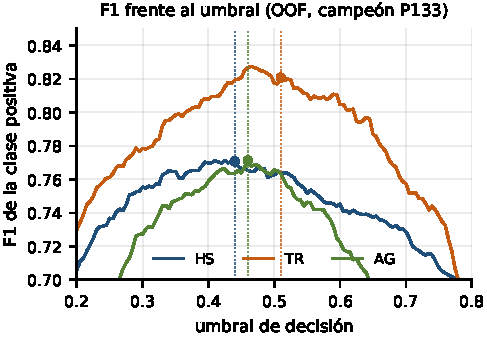
\includegraphics[width=\columnwidth]{fig_umbrales.pdf}
\caption{$F_1$ por etiqueta en función del umbral de decisión (OOF,
campeón P133). Las líneas verticales punteadas marcan los umbrales
congelados; los puntos, el valor que producen. Las mesetas son amplias, lo
que hace que el umbral exacto no sea crítico.}
\label{fig:umbrales}
\end{figure}

\subsection{Análisis de error}

La Tabla~\ref{tab:error} desglosa la matriz de confusión y el desempeño por
longitud. La Figura~\ref{fig:confusion} muestra las matrices de confusión
resultantes. De las tres columnas, TR obtiene el mayor $F_1$ (0.8207): el umbral
alto y el
ancla de positivos compensan su menor prevalencia. HS y AG quedan en 0.7707 y
0.7713, con 175 y 126 falsos positivos y 132 falsos negativos cada una. El
patrón por longitud es el hallazgo más claro: los tuits cortos alcanzan
0.8824, los medios 0.7544 y los largos 0.6306. La caída no es solo de
vocabulario: los textos largos contienen más contexto, más ironía y más
discurso citado, y el modelo lineal, que decide por suma de indicios, pierde
precisión cuando el contexto cambia el signo de una palabra.

\begin{table}[t]
\centering
\caption{Análisis de error del campeón. Arriba: matriz de confusión por
etiqueta (OOF). Abajo: $F_1$ por franja de longitud; los cortes son los
terciles de 70 y 118 caracteres.}
\label{tab:error}
\small
\begin{tabular}{lrrrrr}
\toprule
Etiqueta & TP & FP & FN & TN & $F_1$ \\
\midrule
HS & 516 & 175 & 132 & 660 & 0.7707 \\
TR & 364 & 78 & 81 & 960 & 0.8207 \\
AG & 435 & 126 & 132 & 790 & 0.7713 \\
\midrule
Franja & $n$ & Macro & HS & TR & AG \\
\midrule
Corta ($\le 70$) & 504 & 0.8824 & 0.8633 & 0.9000 & 0.8840 \\
Media ($71$--$118$) & 488 & 0.7544 & 0.7560 & 0.7742 & 0.7331 \\
Larga ($>118$) & 491 & 0.6306 & 0.6466 & 0.6250 & 0.6202 \\
\bottomrule
\end{tabular}
\end{table}

\begin{figure*}[t]
\centering
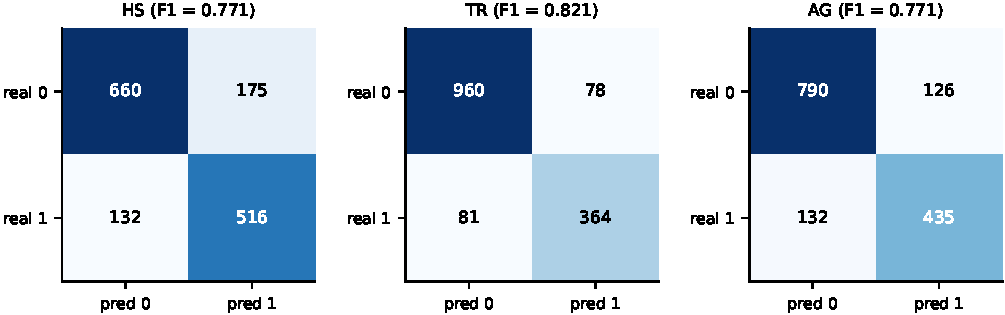
\includegraphics[width=\textwidth]{fig_confusion.pdf}
\caption{Matrices de confusión del campeón P133 sobre las predicciones OOF
de la partición canónica. La asimetría entre falsos positivos y falsos
negativos es distinta por etiqueta: HS sobrerrepresenta positivos, AG presenta
un leve sesgo hacia falsos negativos y TR está equilibrada (78/81).}
\label{fig:confusion}
\end{figure*}

El análisis por rebanadas de la fase inicial (sobre las 1\,731 filas y el
modelo V03) identifica las regiones más débiles: los tuits con hashtag
($F_1=0.586$), con pregunta (0.633), con referencia colectiva (0.639), el
cuartil superior de longitud (0.645) y los que no tienen mención (0.697). El
45.5\,\% de los falsos negativos de AG contiene una referencia colectiva,
frente al 13.9\,\% de los verdaderos positivos: la agresividad que se escapa
es, sobre todo, contra grupos. El régimen de respuesta con mención inicial
alcanza $F_1=0.876$, mientras que el régimen de noticia o atribución se queda
en 0.702. Estas cifras fijan el techo práctico del enfoque y orientan el
trabajo futuro.

Los errores residuales se agrupan en cuatro patrones. Primero, falsos
positivos léxicos: palabras vulgares en contextos inocentes (mascotas,
canciones, elogios, bromas entre amigos). Segundo, falsos negativos de odio
implícito: deshumanización o exclusión sin insulto del léxico vigilado.
Tercero, desacuerdos de anotación en TR, sobre todo cuando la definición de
la competencia y la de HatEval difieren. Cuarto, discurso citado o narrativo:
el tuit reproduce un insulto ajeno y el modelo lo atribuye al autor. Los
ejemplos se presentan enmascarados en el cuaderno para no reproducir el
contenido ofensivo. La consecuencia práctica es que buena parte del error
restante no es un problema de capacidad del modelo, sino de ambigüedad
semántica y de definición de la etiqueta.

\subsection{Validez externa y riesgo de sobreajuste al leaderboard}

La lectura honesta de los resultados exige separar dos cosas. El modelo base
se validó con particiones agrupadas, bootstrap y McNemar; su mejora sobre V03
es la parte que generalizaría a datos nuevos. La capa de pares compensados no
se validó así: sus reglas se diseñaron para textos concretos del test, con
cero coincidencias en entrenamiento, y se aceptaron o rechazaron con el
leaderboard público. Es una forma de adaptación al test, legítima dentro de
las reglas de la competencia, pero distinta de la generalización.

El riesgo es real. Con 47 envíos de modelos al leaderboard (más la sonda de
plantilla; 25 de esta serie) y un
leaderboard público fijo, la búsqueda adaptativa puede encontrar reglas que
mejoran esa muestra y no el conjunto privado. La incertidumbre marginal de la
métrica es apreciable: el error estándar bootstrap agrupado de la $F_1$ del
campeón en desarrollo es 0.0117; escalado al tamaño del test (1\,154), del
orden de 0.013. Las diferencias de 0.001--0.005 solo son interpretables porque
son pareadas y porque cada envío cambia un lote contable. La Figura~\ref{fig:bootstrap} resume las mejoras
locales y el desempeño por franja de longitud. La literatura sobre
holdouts reutilizables advierte que la adaptación repetida al mismo conjunto
puede inflar el resultado \cite{dwork2015reusable}. Varias salvaguardas
reducen el riesgo: los lotes preservan el número de positivos por columna, las
firmas léxicas son específicas, cada envío se audita antes de subirse y la
decisión se registra con su delta. Aun así, no eliminan el riesgo. El
leaderboard privado es la prueba final y, a la fecha de este informe, no se
conoce.

La consecuencia para el artículo es que el 0.81447 no debe leerse como una
estimación insesgada de la $F_1$ en población. Es el resultado de un sistema
en una competencia, con una capa de decisión adaptada al test. La estimación
limpia es la del modelo base: 0.787582 OOF, con IC95 para la mejora sobre
V03. Ambas cifras son ciertas; miden cosas distintas. Presentarlas separadas
es más informativo que quedarse con la más alta.

\subsection{Comparación con la literatura y límites}

Los sistemas clásicos de HatEval combinaron rasgos lingüísticos, n-gramas y
modelos lineales o neuronales, y muchos quedaron en el rango de 0.70--0.80 de
$F_1$ en español \cite{basile2019hateval,argotavega2019mineriaunam,ninaalcocer2019haterecognizer,pereirakohatsu2019haternet}.
Nuestro modelo base es coherente con esa familia y añade una ingeniería de
representación y decisión que lo lleva a la parte alta del rango, aunque la
comparación entre corpus no es directa. Los
transformers habrían sido la alternativa natural, pero estaban prohibidos; la
comparación directa con ellos no es posible en este contexto
\cite{plazadelarco2021comparing}. La capa de pares compensados es ortogonal
al modelo: podría aplicarse a cualquier base, siempre que se acepte su costo
de adaptación al test.

Los límites son claros. El corpus es pequeño (1\,731 filas), de un solo
idioma, normalizado a ASCII y con ruido de anotación; los near-duplicados se
mitigan con grupos, pero no desaparecen; la definición de TR es ambigua; y
la selección de 25 candidatos en el leaderboard introduce un sesgo de
selección que el bootstrap local no captura. No hubo validación externa ni
evaluación prospectiva. Estas limitaciones no invalidan el resultado, pero
acotan su alcance: es un sistema de competencia, reproducible y auditado, no
un clasificador listo para producción.

\begin{figure*}[t]
\centering
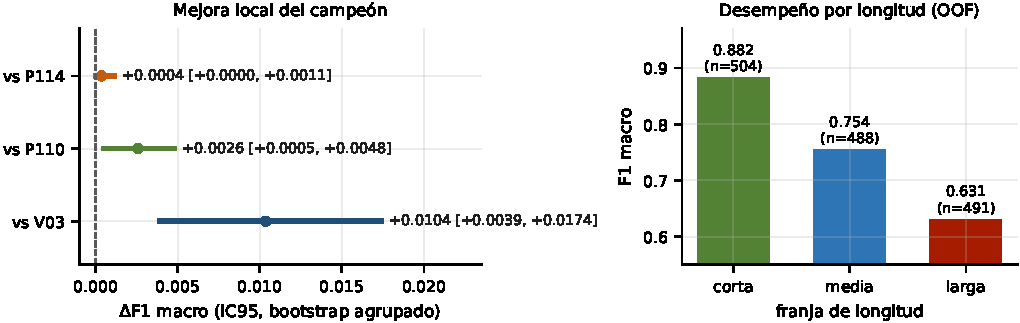
\includegraphics[width=\textwidth]{fig_bootstrap.pdf}
\caption{Izquierda: mejora local del campeón frente a V03, P110 y P114, con
IC95 por bootstrap agrupado. Derecha: $F_1$ macro por franja de longitud; la
caída en los textos largos es el principal frente de mejora.}
\label{fig:bootstrap}
\end{figure*}

\section{Reproducibilidad y despliegue}
\label{sec:reproducibilidad}

\subsection{Entrenamiento final y envío}

El envío campeón se produce con un protocolo distinto al de la validación: los
tres modelos del ensamble se reajustan para cada etiqueta (nueve clasificadores
binarios) sobre las 1\,731 filas de entrenamiento, sin submuestreo ni bagging, y
se combinan con los pesos 80/5/15 y la temperatura 1.04. Sobre las
probabilidades calibradas se aplica la cadena completa de staging (la base
P121/P122 más los lotes aceptados P124--P128 y P131--P133), los umbrales
0.44/0.51/0.46 y la regla ascendente. El resultado se escribe en
\texttt{submission.csv} y se audita antes de subirlo.

Dos celdas del test quedan históricamente a menos de $5\times10^{-4}$ de su
umbral: el tuit con id 24341 en HS (probabilidad 0.439698, margen
$-3.02\times10^{-4}$) y el tuit con id 23726 en TR (0.509755,
$-2.45\times10^{-4}$). En el entorno de
referencia su decisión es estable, pero versiones distintas de
\texttt{scikit-learn} pueden invertirlas por diferencias de punto flotante en
el solver SAGA \cite{defazio2014saga}. Para que el envío sea invariante al
entorno, el cuaderno fija esas dos celdas a la decisión oficial registrada y
presenta una auditoría con la probabilidad viva, el umbral y el margen. Las
otras 3\,460 celdas se calculan en vivo. El protocolo no oculta nada: la
auditoría se imprime en la ejecución y las dos celdas se identifican por su
\texttt{id}.

\subsection{Verificación criptográfica e idempotencia}

El envío tiene 1\,154 filas, las columnas \texttt{id, HS, TR, AG} en el orden
correcto, 514 positivos en HS, 330 en TR y 421 en AG (1\,265 en total,
36.54\,\%), se aplicaron ocho correcciones ascendentes ($TR=1$, $HS=0$) y,
tras ellas, cero violaciones de la regla HatEval. Su SHA256 es
\begin{center}
\texttt{\scriptsize b0979a8ac51074daa2543f97944a499d9}\\
\texttt{\scriptsize c61cf9f38bcd094f510550b184079fe}
\end{center}
El cuaderno se ejecutó dos veces de principio a fin en máquinas limpias; ambas
corridas produjeron el mismo archivo y la misma huella. Además, la cadena de
staging reproduce bit a bit los envíos oficiales de P128, P131, P132 y P133
cuando se le dan las probabilidades de referencia del test: 0 celdas
distintas en los cuatro casos. Esa regresión es la prueba más fuerte de que
la implementación publicada y el envío histórico son el mismo objeto.

\begin{table}[t]
\centering
\caption{Verificaciones de reproducibilidad. Los SHA se muestran con sus
primeros 16 caracteres; el SHA completo del campeón está en el texto.}
\label{tab:repro}
\small
\begin{tabular}{ll}
\toprule
Envío & SHA256 (16 primeros) \\
\midrule
P128 & \texttt{ef3d694988ebe945} \\
P131 & \texttt{e10bc59682a5c62b} \\
P132 & \texttt{9207779494f0f42e} \\
P133 & \texttt{b0979a8ac51074da} \\
\midrule
Comprobación & Resultado \\
\midrule
Filas & 1\,154 \\
Ancla HS/TR/AG & 514 / 330 / 421 \\
Total de positivos & 1\,265 (36.54\,\%) \\
Violaciones HatEval & 0 \\
Celdas de frontera & 2 de 3\,462 \\
Idempotencia & 2 corridas, mismo SHA \\
\bottomrule
\end{tabular}
\end{table}

\subsection{Artefactos y entorno}

El cuaderno autocontenido (\texttt{kaggle\_}\allowbreak\texttt{final\_}\allowbreak\texttt{pipeline.ipynb},
ubicado en \path{notebooks/}) localiza los CSV de la competencia, reconstruye las particiones, entrena el
banco de probabilidades, re-ejecuta la serie P108--P133, aplica el staging y
verifica el SHA. Se ejecutó con el kernel de referencia del proyecto
(\texttt{numpy} 1.26.4, \texttt{scipy} 1.17.1, \texttt{scikit-learn} 1.8.0
\cite{pedregosa2011scikit}, \texttt{pandas} 2.3.3) y con las semillas fijas (42 en modelos y pliegues,
20260925 en bootstrap). Los scripts de cada experimento, los reportes con sus
métricas y el registro \texttt{experiments.csv} (532 filas) acompañan al
cuaderno; el anexo del cuaderno reúne las 565 entradas del inventario. La
Tabla~\ref{tab:repro} resume las comprobaciones.

\subsection{Disponibilidad de datos y código}
Los archivos de la competencia no se redistribuyen. El cuaderno
\texttt{kaggle\_}\allowbreak\texttt{final\_}\allowbreak\texttt{pipeline.ipynb}
(en \path{notebooks/}), los scripts de los experimentos,
el registro \texttt{experiments.csv} y el envío campeón están en el repositorio
del proyecto. El cuaderno reconstruye el envío y verifica su SHA256; las
instrucciones de ejecución están en el README del informe.

\section{Conclusiones y trabajo futuro}
\label{sec:conclusiones}

La pregunta que abrió este artículo tenía una respuesta afirmativa, aunque
con matices. Un pipeline clásico, sin transformers ni representaciones
preentrenadas, puede competir en un corpus pequeño y ruidoso de tuits en
español si se cuidan tres cosas: la representación, la validación y la
decisión. El sistema alcanzó un $F_1$ público de 0.81447 y el primer lugar
del leaderboard al cierre de este informe. La estimación limpia de su
capacidad de generalización es, sin embargo, la del modelo base: 0.787582
out-of-fold, con una mejora de $+0.010370$ sobre V03 e IC95
$[+0.003924, +0.017386]$. Las dos cifras miden cosas distintas y ambas deben
reportarse.

La primera lección es que la representación sigue importando. La unión
multiescala de palabras y n-gramas de caracteres aportó $+0.00516$ local y
$+0.00549$ en el leaderboard, y lo hizo en las dos particiones congeladas.
En un corpus normalizado a ASCII, corto y con ruido ortográfico, los
n-gramas de caracteres no son un adorno: son el mecanismo que recupera la
morfología y la jerga que el vocabulario de palabras pierde.

La segunda lección es que la validación puede inducir a error si se diseña mal. P109
obtuvo la mejor métrica local de toda la serie y el peor resultado público.
La causa fue la poda por frecuencia: el vocabulario se hizo más pequeño,
la validación compartió esa estrechez y el test no. La validación agrupada,
la réplica en dos particiones y los controles de determinismo no eliminan el
problema, pero lo hacen visible. Sin ellos, P109 habría parecido el mejor
modelo del proyecto.

La tercera lección es que la capa de decisión tiene una economía propia. La
Proposición~\ref{prop:par} demuestra que un par compensado incrementa la
$F_1$ en $F_1/TP$ por columna y preserva el número de positivos. Esa fórmula
predice por qué los pares funcionan, por qué TR es la columna más sensible y
por qué P129 falló al saturar la probabilidad. También explica por qué la
capa no se puede validar con la OOF: sus reglas se diseñaron para textos del
test. El 76\,\% de la ganancia del leaderboard proviene de ahí, y esa es
precisamente la parte que exige más cautela.

El trabajo futuro tiene cuatro frentes. Primero, repetir el pipeline con
transformers o modelos de lenguaje, si las reglas lo permiten, para medir
cuánto de la brecha es representación y cuánto es arquitectura. Segundo,
atacar el error residual con mejor etiquetado y con modelos que manejen
ironía, discurso citado y odio implícito; el análisis por longitud muestra
que los textos largos son el frente principal. Tercero, diseñar una capa de
decisión que no dependa del leaderboard: calibración con validación
prospectiva, abstención cuando la probabilidad está cerca del umbral y
auditoría de subgrupos. Cuarto, evaluar el sistema con criterios de equidad
y robustez antes de pensar en un despliegue real; la literatura sobre sesgos
en corpus de odio es una advertencia que este trabajo no resuelve
\cite{davidson2019racial,wiegand2019biased}.

El resultado que queda es moderado pero significativo. Moderado porque
0.81447 es el puntaje de una competencia, con una capa adaptada al test y un
leaderboard privado que aún no se conoce. Significativo porque demuestra que
una representación construida desde cero, un ensamble lineal bien calibrado
y una capa de decisión auditable pueden llevar a un sistema clásico hasta el
primer lugar. En un momento en que la alternativa por defecto son los transformers, este
caso recuerda que la ingeniería de datos, la validación y
la teoría de la decisión siguen siendo fuentes reales de mejora.


\clearpage
\appendix[Inventario completo de la experimentación]
\label{app:inventario}

\begin{table*}[!t]
\centering
\caption{Inventario agrupado de las 565 entradas. Los conteos incluyen
experimentos, auditorías y scripts de apoyo; la lista completa de
identificadores está en la Subsección~\ref{subsec:lista}.}
\label{tab:inventario}
\scriptsize
\begin{tabularx}{\textwidth}{@{}>{\raggedright\arraybackslash}p{4.2cm}r>{\raggedright\arraybackslash}X>{\raggedright\arraybackslash}p{2.8cm}@{}}
\toprule
Grupo & $n$ & Resultado principal & Decisión \\
\midrule
Preparación y baseline & 32 & E00 0.5149; B1 0.7587/0.7568; MOD-03b 0.7927; DL 0.7949; densos $-0.009$ a $-0.032$. & V03 base; resto descartado. \\
Fases v1--v44 & 167 & V03 0.7772/0.7831; meseta 0.7772--0.7927; sin transferencia. & V03 adoptado. \\
Auditorías P45--P59 & 10 & Sin mejora de modelo. & Cerradas. \\
Auditorías P60--P68 & 56 & Sin transferencia. & Cerradas. \\
Auditorías P69--P77 & 37 & Mejor $+0.0023$ anidado; LB sin mejora. & Descartadas. \\
Auditorías P78--P84 & 12 & Sin adopción. & Cerradas. \\
Embeddings y corpus P85--P100 & 62 & FastText 0.652--0.653 OOF; fusión $+0.0046$ (IC cruza 0); sin LB. & Rechazado. \\
Cierre P101--P107 & 15 & Sin mejora de modelo. & Cerrado. \\
Serie final P108--P133 & 26 & 0.7886 $\to$ 0.8145; 25 LB; P133 final. & Adoptado. \\
Fases v45--v58 y auditorías & 148 & Cierres y auditorías; V47 0.7718 sin adopción. & Cerrado. \\
\bottomrule
\end{tabularx}
\end{table*}

El registro del proyecto contiene 565 entradas: 532 filas de
\texttt{experiments.csv} y 33 entradas del inventario de auditoría. De ellas,
353 tienen fuente y resultado, 196 son auxiliares y 16 son documentales; 552
scripts están en \texttt{experiments/}. La Tabla~\ref{tab:inventario} las
agrupa por fase y resume el resultado principal de cada grupo; la
Subsección~\ref{subsec:lista} presenta la lista completa de identificadores.
El detalle de estado, fuente, resultado y observación está en
\texttt{auditoria/auditoria\_\allowbreak{}experimentos.csv}.



La tabla se lee como un mapa, no como un sustituto del registro. Las fases
tempranas y las auditorías ocuparon la mayor parte del esfuerzo y dejaron un
catálogo de resultados negativos; la serie final concentró las decisiones que
cambiaron la métrica. El patrón es consistente con la
Sección~\ref{sec:arquitectura}: la representación y el modelo base aportaron
$+0.00751$ y la capa de decisión, $+0.02390$; el resto de las alternativas no
pasó la barrera de adopción o no transfirió al leaderboard.

\subsection{Lista completa de identificadores}
\label{subsec:lista}

La lista se ordena por fase y, dentro de cada fase, alfabéticamente. Los
identificadores se muestran en \texttt{fuente monoespaciada}; los que contienen
guiones bajos se escapan para LaTeX. La unión es la del registro oficial y el
inventario de auditoría; no se repite ningún identificador.

\begin{multicols}{2}
\raggedright
\scriptsize
\noindent\textbf{Preparación, baseline y modelos tempranos} (32): \texttt{B1}, \texttt{B5-\allowbreak{}DENSE}, \texttt{DL-\allowbreak{}01}, \texttt{DL-\allowbreak{}01-\allowbreak{}SEEDS}, \texttt{DL-\allowbreak{}02}, \texttt{DL-\allowbreak{}03}, \texttt{E00}, \texttt{MOD-\allowbreak{}01\_\allowbreak{}BEST}, \texttt{MOD-\allowbreak{}01\_\allowbreak{}W12}, \texttt{MOD-\allowbreak{}02\_\allowbreak{}BEST}, \texttt{MOD-\allowbreak{}02\_\allowbreak{}W12}, \texttt{MOD-\allowbreak{}03a\_\allowbreak{}BEST}, \texttt{MOD-\allowbreak{}03a\_\allowbreak{}W12}, \texttt{MOD-\allowbreak{}03b\_\allowbreak{}BEST}, \texttt{MOD-\allowbreak{}03b\_\allowbreak{}W12}, \texttt{MOD-\allowbreak{}04}, \texttt{PRE-\allowbreak{}00}, \texttt{PRE-\allowbreak{}01}, \texttt{PRE-\allowbreak{}02}, \texttt{PRE-\allowbreak{}03}, \texttt{PRE-\allowbreak{}04}, \texttt{PRE-\allowbreak{}05}, \texttt{PRE-\allowbreak{}06}, \texttt{PRE-\allowbreak{}07}, \texttt{PRE-\allowbreak{}08}, \texttt{PRE-\allowbreak{}09}, \texttt{REP-\allowbreak{}01}, \texttt{REP-\allowbreak{}02}, \texttt{REP-\allowbreak{}03}, \texttt{REP-\allowbreak{}04}, \texttt{REP-\allowbreak{}05}, \texttt{REP-\allowbreak{}06}\par\smallskip
\noindent\textbf{Fases v1--v44} (167): \texttt{V10-\allowbreak{}00}, \texttt{V10-\allowbreak{}01}, \texttt{V10-\allowbreak{}02}, \texttt{V10-\allowbreak{}03}, \texttt{V10-\allowbreak{}04}, \texttt{V10-\allowbreak{}05}, \texttt{V10-\allowbreak{}06}, \texttt{V10-\allowbreak{}07}, \texttt{V10-\allowbreak{}08}, \texttt{V10-\allowbreak{}09}, \texttt{V10-\allowbreak{}10}, \texttt{V10-\allowbreak{}11}, \texttt{V11-\allowbreak{}00}, \texttt{V11-\allowbreak{}01}, \texttt{V11-\allowbreak{}02}, \texttt{V11-\allowbreak{}03}, \texttt{V11-\allowbreak{}05}, \texttt{V11-\allowbreak{}06}, \texttt{V11-\allowbreak{}07}, \texttt{V11-\allowbreak{}08}, \texttt{V11-\allowbreak{}09}, \texttt{V12-\allowbreak{}00}, \texttt{V12-\allowbreak{}01}, \texttt{V12-\allowbreak{}02}, \texttt{V12-\allowbreak{}03}, \texttt{V12-\allowbreak{}04}, \texttt{V12-\allowbreak{}05}, \texttt{V13-\allowbreak{}00}, \texttt{V13-\allowbreak{}01}, \texttt{V13-\allowbreak{}02}, \texttt{V14-\allowbreak{}00}, \texttt{V14-\allowbreak{}01}, \texttt{V15-\allowbreak{}00}, \texttt{V15-\allowbreak{}01}, \texttt{V15-\allowbreak{}02}, \texttt{V16-\allowbreak{}00}, \texttt{V16-\allowbreak{}02}, \texttt{V16-\allowbreak{}03}, \texttt{V17-\allowbreak{}00}, \texttt{V18-\allowbreak{}01}, \texttt{V19-\allowbreak{}00}, \texttt{V19-\allowbreak{}01}, \texttt{V19-\allowbreak{}02}, \texttt{V2-\allowbreak{}BASE-\allowbreak{}M1\_\allowbreak{}word\_\allowbreak{}lr}, \texttt{V2-\allowbreak{}BASE-\allowbreak{}M2\_\allowbreak{}union\_\allowbreak{}lr\_\allowbreak{}c2}, \texttt{V2-\allowbreak{}BASE-\allowbreak{}M3\_\allowbreak{}union\_\allowbreak{}svc}, \texttt{V2-\allowbreak{}BASE-\allowbreak{}M4\_\allowbreak{}char\_\allowbreak{}lr}, \texttt{V20-\allowbreak{}01}, \texttt{V20-\allowbreak{}02}, \texttt{V21-\allowbreak{}01}, \texttt{V24-\allowbreak{}01}, \texttt{V25-\allowbreak{}01}, \texttt{V25-\allowbreak{}02}, \texttt{V26-\allowbreak{}01}, \texttt{V26-\allowbreak{}02}, \texttt{V26-\allowbreak{}03}, \texttt{V27-\allowbreak{}01}, \texttt{V28-\allowbreak{}00}, \texttt{V28-\allowbreak{}01}, \texttt{V28-\allowbreak{}03}, \texttt{V28-\allowbreak{}04}, \texttt{V29-\allowbreak{}00}, \texttt{V29-\allowbreak{}01}, \texttt{V29-\allowbreak{}02}, \texttt{V29-\allowbreak{}03}, \texttt{V29-\allowbreak{}04}, \texttt{V29-\allowbreak{}05}, \texttt{V30-\allowbreak{}00}, \texttt{V30-\allowbreak{}01}, \texttt{V30-\allowbreak{}02}, \texttt{V31-\allowbreak{}00}, \texttt{V31-\allowbreak{}01}, \texttt{V31-\allowbreak{}02}, \texttt{V31-\allowbreak{}03}, \texttt{V31-\allowbreak{}04}, \texttt{V31-\allowbreak{}05}, \texttt{V32-\allowbreak{}00}, \texttt{V32-\allowbreak{}01}, \texttt{V32-\allowbreak{}02}, \texttt{V32-\allowbreak{}03}, \texttt{V32-\allowbreak{}04}, \texttt{V32-\allowbreak{}05}, \texttt{V32-\allowbreak{}06}, \texttt{V32-\allowbreak{}07}, \texttt{V33-\allowbreak{}00}, \texttt{V33-\allowbreak{}01}, \texttt{V33-\allowbreak{}02}, \texttt{V33-\allowbreak{}03}, \texttt{V33-\allowbreak{}04}, \texttt{V34-\allowbreak{}01}, \texttt{V34-\allowbreak{}02}, \texttt{V35-\allowbreak{}00}, \texttt{V35-\allowbreak{}01}, \texttt{V35-\allowbreak{}02}, \texttt{V36-\allowbreak{}00}, \texttt{V36-\allowbreak{}01}, \texttt{V36-\allowbreak{}02}, \texttt{V37-\allowbreak{}00}, \texttt{V37-\allowbreak{}01}, \texttt{V37-\allowbreak{}02}, \texttt{V38-\allowbreak{}00}, \texttt{V38-\allowbreak{}01}, \texttt{V38-\allowbreak{}02}, \texttt{V39-\allowbreak{}00}, \texttt{V39-\allowbreak{}01}, \texttt{V39-\allowbreak{}02}, \texttt{V4-\allowbreak{}00-\allowbreak{}SCAFFOLD}, \texttt{V4-\allowbreak{}A01}, \texttt{V4-\allowbreak{}A02}, \texttt{V4-\allowbreak{}B01}, \texttt{V4-\allowbreak{}B02}, \texttt{V4-\allowbreak{}B03}, \texttt{V4-\allowbreak{}B04}, \texttt{V4-\allowbreak{}B05}, \texttt{V4-\allowbreak{}D01-\allowbreak{}D04}, \texttt{V4-\allowbreak{}E01-\allowbreak{}E03}, \texttt{V4-\allowbreak{}F01-\allowbreak{}F04}, \texttt{V4-\allowbreak{}G01-\allowbreak{}G03}, \texttt{V4-\allowbreak{}H01}, \texttt{V4-\allowbreak{}X01}, \texttt{V40-\allowbreak{}00}, \texttt{V40-\allowbreak{}01}, \texttt{V40-\allowbreak{}02}, \texttt{V41-\allowbreak{}00}, \texttt{V41-\allowbreak{}01}, \texttt{V42-\allowbreak{}00}, \texttt{V42-\allowbreak{}01}, \texttt{V43-\allowbreak{}00}, \texttt{V43-\allowbreak{}01}, \texttt{V43-\allowbreak{}02}, \texttt{V44-\allowbreak{}00}, \texttt{V44-\allowbreak{}01}, \texttt{V44-\allowbreak{}02}, \texttt{V44-\allowbreak{}03}, \texttt{V6-\allowbreak{}00}, \texttt{V6-\allowbreak{}01}, \texttt{V6-\allowbreak{}02}, \texttt{V6-\allowbreak{}03}, \texttt{V6-\allowbreak{}04}, \texttt{V6-\allowbreak{}05}, \texttt{V6-\allowbreak{}06}, \texttt{V6-\allowbreak{}07}, \texttt{V6-\allowbreak{}08}, \texttt{V6-\allowbreak{}09}, \texttt{V7-\allowbreak{}01}, \texttt{V7-\allowbreak{}02}, \texttt{V7-\allowbreak{}03}, \texttt{V7-\allowbreak{}04}, \texttt{V8-\allowbreak{}00}, \texttt{V8-\allowbreak{}01}, \texttt{V8-\allowbreak{}02}, \texttt{V8-\allowbreak{}03}, \texttt{V8-\allowbreak{}04}, \texttt{V8-\allowbreak{}05}, \texttt{V8-\allowbreak{}06}, \texttt{V8-\allowbreak{}07}, \texttt{V8-\allowbreak{}08}, \texttt{V8-\allowbreak{}09}, \texttt{V8-\allowbreak{}10}, \texttt{V8-\allowbreak{}11}, \texttt{V8-\allowbreak{}12}, \texttt{V8-\allowbreak{}13}, \texttt{V9-\allowbreak{}01}, \texttt{V9-\allowbreak{}02}, \texttt{V9-\allowbreak{}03}, \texttt{V9-\allowbreak{}04}, \texttt{V9-\allowbreak{}05}\par\smallskip
\noindent\textbf{Auditorías P45--P59} (10): \texttt{P59-\allowbreak{}01}, \texttt{P59-\allowbreak{}02}, \texttt{P59-\allowbreak{}05}, \texttt{P59-\allowbreak{}06}, \texttt{P59-\allowbreak{}07}, \texttt{P59-\allowbreak{}08}, \texttt{P59-\allowbreak{}09}, \texttt{P59-\allowbreak{}10}, \texttt{P59-\allowbreak{}11}, \texttt{P8-\allowbreak{}REFIT-\allowbreak{}C}\par\smallskip
\noindent\textbf{Auditorías P60--P68} (56): \texttt{P60-\allowbreak{}01}, \texttt{P60-\allowbreak{}02}, \texttt{P60-\allowbreak{}03}, \texttt{P60-\allowbreak{}04}, \texttt{P60-\allowbreak{}05}, \texttt{P60-\allowbreak{}05-\allowbreak{}RUIDO-\allowbreak{}POR-\allowbreak{}ETIQUETA}, \texttt{P60-\allowbreak{}06}, \texttt{P60-\allowbreak{}07}, \texttt{P60-\allowbreak{}08}, \texttt{P61-\allowbreak{}01}, \texttt{P61-\allowbreak{}01-\allowbreak{}EDA-\allowbreak{}PROBABILIDADES}, \texttt{P61-\allowbreak{}02}, \texttt{P61-\allowbreak{}02-\allowbreak{}INVENTARIO}, \texttt{P61-\allowbreak{}03}, \texttt{P62-\allowbreak{}01}, \texttt{P62-\allowbreak{}02}, \texttt{P62-\allowbreak{}03}, \texttt{P62-\allowbreak{}04}, \texttt{P62-\allowbreak{}05}, \texttt{P62-\allowbreak{}10}, \texttt{P63-\allowbreak{}00}, \texttt{P63-\allowbreak{}01}, \texttt{P63-\allowbreak{}02}, \texttt{P63-\allowbreak{}03}, \texttt{P63-\allowbreak{}04}, \texttt{P63-\allowbreak{}04C}, \texttt{P63-\allowbreak{}05}, \texttt{P63-\allowbreak{}06}, \texttt{P63-\allowbreak{}06C}, \texttt{P63-\allowbreak{}07}, \texttt{P63-\allowbreak{}09}, \texttt{P64-\allowbreak{}00}, \texttt{P64-\allowbreak{}01}, \texttt{P64-\allowbreak{}02}, \texttt{P64-\allowbreak{}03}, \texttt{P64-\allowbreak{}04}, \texttt{P64-\allowbreak{}05}, \texttt{P64-\allowbreak{}06}, \texttt{P64-\allowbreak{}07}, \texttt{P64-\allowbreak{}08}, \texttt{P65-\allowbreak{}00}, \texttt{P65-\allowbreak{}01}, \texttt{P65-\allowbreak{}02}, \texttt{P65-\allowbreak{}03}, \texttt{P65-\allowbreak{}04}, \texttt{P66-\allowbreak{}00}, \texttt{P66-\allowbreak{}01}, \texttt{P66-\allowbreak{}02}, \texttt{P66-\allowbreak{}03}, \texttt{P67-\allowbreak{}00}, \texttt{P67-\allowbreak{}01}, \texttt{P67-\allowbreak{}02}, \texttt{P67-\allowbreak{}03}, \texttt{P67-\allowbreak{}04}, \texttt{P68-\allowbreak{}01}, \texttt{P68-\allowbreak{}02}\par\smallskip
\noindent\textbf{Auditorías P69--P77} (37): \texttt{P69-\allowbreak{}01}, \texttt{P69-\allowbreak{}02}, \texttt{P69-\allowbreak{}03}, \texttt{P69-\allowbreak{}04}, \texttt{P69-\allowbreak{}05}, \texttt{P69-\allowbreak{}06}, \texttt{P69-\allowbreak{}07}, \texttt{P69-\allowbreak{}08}, \texttt{P69-\allowbreak{}09}, \texttt{P69-\allowbreak{}10}, \texttt{P70-\allowbreak{}01}, \texttt{P70-\allowbreak{}02}, \texttt{P70-\allowbreak{}03}, \texttt{P71-\allowbreak{}00}, \texttt{P71-\allowbreak{}01}, \texttt{P71-\allowbreak{}02}, \texttt{P71-\allowbreak{}03}, \texttt{P71-\allowbreak{}04}, \texttt{P71-\allowbreak{}05}, \texttt{P71-\allowbreak{}06}, \texttt{P71-\allowbreak{}07}, \texttt{P71-\allowbreak{}08}, \texttt{P71-\allowbreak{}09}, \texttt{P71-\allowbreak{}10}, \texttt{P72-\allowbreak{}00}, \texttt{P72-\allowbreak{}01}, \texttt{P72-\allowbreak{}02}, \texttt{P72-\allowbreak{}03}, \texttt{P72-\allowbreak{}04}, \texttt{P73-\allowbreak{}01}, \texttt{P73-\allowbreak{}02}, \texttt{P73-\allowbreak{}03}, \texttt{P74}, \texttt{P74-\allowbreak{}PRE}, \texttt{P75}, \texttt{P76}, \texttt{P77}\par\smallskip
\noindent\textbf{Auditorías P78--P84} (12): \texttt{P78}, \texttt{P79}, \texttt{P80}, \texttt{P81}, \texttt{P82}, \texttt{P82-\allowbreak{}02}, \texttt{P83}, \texttt{P84-\allowbreak{}01}, \texttt{P84-\allowbreak{}02}, \texttt{P84-\allowbreak{}03}, \texttt{P84-\allowbreak{}04}, \texttt{P84-\allowbreak{}05}\par\smallskip
\noindent\textbf{Embeddings y corpus P85--P100} (62): \texttt{EBD-\allowbreak{}00-\allowbreak{}SCAFFOLD}, \texttt{EBD-\allowbreak{}01}, \texttt{EBD-\allowbreak{}02}, \texttt{EBD-\allowbreak{}03}, \texttt{EBD-\allowbreak{}04}, \texttt{EBD-\allowbreak{}05}, \texttt{EBD-\allowbreak{}06}, \texttt{EBD-\allowbreak{}07}, \texttt{EBD-\allowbreak{}08}, \texttt{EBD-\allowbreak{}09}, \texttt{EBD-\allowbreak{}10}, \texttt{EBD-\allowbreak{}13}, \texttt{EBD-\allowbreak{}14}, \texttt{EBD-\allowbreak{}15}, \texttt{EBD-\allowbreak{}16}, \texttt{EBD-\allowbreak{}17}, \texttt{EBD-\allowbreak{}18}, \texttt{EBD-\allowbreak{}19}, \texttt{EBD-\allowbreak{}20}, \texttt{EBD-\allowbreak{}21}, \texttt{EBD-\allowbreak{}22}, \texttt{EBD-\allowbreak{}23}, \texttt{EBD-\allowbreak{}24}, \texttt{EBD-\allowbreak{}25}, \texttt{EBD-\allowbreak{}26}, \texttt{EBD-\allowbreak{}27}, \texttt{P100-\allowbreak{}00}, \texttt{P100-\allowbreak{}10}, \texttt{P100-\allowbreak{}11}, \texttt{P100-\allowbreak{}12}, \texttt{P100-\allowbreak{}13}, \texttt{P100-\allowbreak{}14}, \texttt{P85-\allowbreak{}01}, \texttt{P86-\allowbreak{}00}, \texttt{P87-\allowbreak{}00}, \texttt{P88-\allowbreak{}00}, \texttt{P97-\allowbreak{}00}, \texttt{P97-\allowbreak{}01}, \texttt{P97-\allowbreak{}01C}, \texttt{P97-\allowbreak{}02}, \texttt{P97-\allowbreak{}02-\allowbreak{}INV1}, \texttt{P97-\allowbreak{}02C}, \texttt{P97-\allowbreak{}03}, \texttt{P97-\allowbreak{}03-\allowbreak{}INV1}, \texttt{P97-\allowbreak{}03-\allowbreak{}INV2}, \texttt{P97-\allowbreak{}03C}, \texttt{P97-\allowbreak{}04}, \texttt{P97-\allowbreak{}04C}, \texttt{P98-\allowbreak{}00}, \texttt{P98-\allowbreak{}01}, \texttt{P98-\allowbreak{}02}, \texttt{P98-\allowbreak{}10}, \texttt{P98-\allowbreak{}11}, \texttt{P98-\allowbreak{}12}, \texttt{P98-\allowbreak{}13}, \texttt{P98-\allowbreak{}14}, \texttt{P98-\allowbreak{}15}, \texttt{P99-\allowbreak{}00}, \texttt{P99-\allowbreak{}11}, \texttt{P99-\allowbreak{}12}, \texttt{P99-\allowbreak{}13}, \texttt{P99-\allowbreak{}14}\par\smallskip
\noindent\textbf{Cierre P101--P107} (15): \texttt{P101-\allowbreak{}00}, \texttt{P102-\allowbreak{}01}, \texttt{P102-\allowbreak{}02}, \texttt{P102-\allowbreak{}03}, \texttt{P102-\allowbreak{}04}, \texttt{P103-\allowbreak{}01}, \texttt{P103-\allowbreak{}02}, \texttt{P104-\allowbreak{}01}, \texttt{P104-\allowbreak{}02}, \texttt{P104-\allowbreak{}03}, \texttt{P105-\allowbreak{}01}, \texttt{P105-\allowbreak{}02}, \texttt{P105-\allowbreak{}03}, \texttt{P106-\allowbreak{}01}, \texttt{P107-\allowbreak{}01}\par\smallskip
\noindent\textbf{Serie final P108--P133} (26): \texttt{P108-\allowbreak{}01}, \texttt{P109-\allowbreak{}01}, \texttt{P110-\allowbreak{}01}, \texttt{P111-\allowbreak{}01}, \texttt{P112-\allowbreak{}01}, \texttt{P113-\allowbreak{}01}, \texttt{P114-\allowbreak{}01}, \texttt{P115-\allowbreak{}01}, \texttt{P116-\allowbreak{}01}, \texttt{P117-\allowbreak{}01}, \texttt{P118-\allowbreak{}01}, \texttt{P119-\allowbreak{}01}, \texttt{P120-\allowbreak{}01}, \texttt{P121-\allowbreak{}01}, \texttt{P122-\allowbreak{}01}, \texttt{P123-\allowbreak{}01}, \texttt{P124-\allowbreak{}01}, \texttt{P125-\allowbreak{}01}, \texttt{P126-\allowbreak{}01}, \texttt{P127-\allowbreak{}01}, \texttt{P128-\allowbreak{}01}, \texttt{P129-\allowbreak{}01}, \texttt{P130-\allowbreak{}01}, \texttt{P131-\allowbreak{}01}, \texttt{P132-\allowbreak{}01}, \texttt{P133-\allowbreak{}01}\par\smallskip
\noindent\textbf{Fases v45--v58 y auditorías transversales} (148): \texttt{37\_\allowbreak{}auditoria\_\allowbreak{}v4}, \texttt{AUD-\allowbreak{}01}, \texttt{AUD-\allowbreak{}02}, \texttt{AUD-\allowbreak{}03}, \texttt{E-\allowbreak{}CORP-\allowbreak{}01}, \texttt{E-\allowbreak{}CORP-\allowbreak{}06}, \texttt{E-\allowbreak{}CORP-\allowbreak{}07}, \texttt{E-\allowbreak{}CORP-\allowbreak{}08}, \texttt{E-\allowbreak{}CORP-\allowbreak{}09}, \texttt{E2-\allowbreak{}01-\allowbreak{}AG-\allowbreak{}HS-\allowbreak{}TR}, \texttt{E2-\allowbreak{}01-\allowbreak{}AG-\allowbreak{}HS-\allowbreak{}TR-\allowbreak{}STD}, \texttt{E2-\allowbreak{}01-\allowbreak{}HS-\allowbreak{}AG-\allowbreak{}TR}, \texttt{E2-\allowbreak{}01-\allowbreak{}HS-\allowbreak{}AG-\allowbreak{}TR-\allowbreak{}STD}, \texttt{E2-\allowbreak{}01-\allowbreak{}HS-\allowbreak{}TR-\allowbreak{}AG}, \texttt{E2-\allowbreak{}01-\allowbreak{}HS-\allowbreak{}TR-\allowbreak{}AG-\allowbreak{}STD}, \texttt{E2-\allowbreak{}02-\allowbreak{}META}, \texttt{E2-\allowbreak{}03-\allowbreak{}POS}, \texttt{E2-\allowbreak{}03-\allowbreak{}POS-\allowbreak{}TXT}, \texttt{E2-\allowbreak{}04-\allowbreak{}DEPS}, \texttt{E2-\allowbreak{}04-\allowbreak{}DEPS-\allowbreak{}TXT}, \texttt{E2-\allowbreak{}04-\allowbreak{}MORPH}, \texttt{E2-\allowbreak{}04-\allowbreak{}MORPH-\allowbreak{}TXT}, \texttt{E2-\allowbreak{}04-\allowbreak{}SYN3}, \texttt{E2-\allowbreak{}04-\allowbreak{}SYN3-\allowbreak{}TXT}, \texttt{E2-\allowbreak{}05-\allowbreak{}CH-\allowbreak{}TGT}, \texttt{E2-\allowbreak{}05-\allowbreak{}CH-\allowbreak{}TGT-\allowbreak{}DIST}, \texttt{E2-\allowbreak{}06-\allowbreak{}TXT-\allowbreak{}CH}, \texttt{E2-\allowbreak{}06-\allowbreak{}TXT-\allowbreak{}TGT-\allowbreak{}SPARSE}, \texttt{E2-\allowbreak{}07-\allowbreak{}CITA}, \texttt{E2-\allowbreak{}07-\allowbreak{}CITA-\allowbreak{}NEG-\allowbreak{}TXT}, \texttt{E2-\allowbreak{}07-\allowbreak{}CITA-\allowbreak{}TXT}, \texttt{E2-\allowbreak{}08-\allowbreak{}NEG}, \texttt{E2-\allowbreak{}08-\allowbreak{}NEG-\allowbreak{}TXT}, \texttt{E2-\allowbreak{}09-\allowbreak{}EMO}, \texttt{E2-\allowbreak{}09-\allowbreak{}EMO-\allowbreak{}EST}, \texttt{E2-\allowbreak{}09-\allowbreak{}EMO-\allowbreak{}LEX}, \texttt{E2-\allowbreak{}09-\allowbreak{}TXT-\allowbreak{}EMO}, \texttt{E2-\allowbreak{}10-\allowbreak{}ORT-\allowbreak{}A}, \texttt{E2-\allowbreak{}10-\allowbreak{}ORT-\allowbreak{}ABCD}, \texttt{E2-\allowbreak{}10-\allowbreak{}ORT-\allowbreak{}AE}, \texttt{E2-\allowbreak{}13-\allowbreak{}ENT-\allowbreak{}SOLO-\allowbreak{}LR}, \texttt{E2-\allowbreak{}13-\allowbreak{}META-\allowbreak{}ENT-\allowbreak{}LR}, \texttt{E2-\allowbreak{}13-\allowbreak{}META-\allowbreak{}ENT-\allowbreak{}RIDGE}, \texttt{E2-\allowbreak{}14-\allowbreak{}MEJOR-\allowbreak{}M2}, \texttt{E2-\allowbreak{}14-\allowbreak{}MEJOR-\allowbreak{}META}, \texttt{E2-\allowbreak{}15-\allowbreak{}NB-\allowbreak{}CHAR}, \texttt{E2-\allowbreak{}15-\allowbreak{}NB-\allowbreak{}WORD}, \texttt{E2-\allowbreak{}15-\allowbreak{}NBSVM}, \texttt{E2-\allowbreak{}15-\allowbreak{}NBSVM-\allowbreak{}SVC}, \texttt{E2-\allowbreak{}16-\allowbreak{}LOCAL-\allowbreak{}SIN-\allowbreak{}SHRINKAGE}, \texttt{E2-\allowbreak{}16-\allowbreak{}MEJOR}, \texttt{E2-\allowbreak{}16-\allowbreak{}SHRINK-\allowbreak{}M100}, \texttt{E2-\allowbreak{}16-\allowbreak{}SHRINK-\allowbreak{}M25}, \texttt{E2-\allowbreak{}16-\allowbreak{}SHRINK-\allowbreak{}M50}, \texttt{E2-\allowbreak{}18-\allowbreak{}META+\allowbreak{}CH}, \texttt{E2-\allowbreak{}18-\allowbreak{}META+\allowbreak{}CH+\allowbreak{}ESTR}, \texttt{E2-\allowbreak{}18-\allowbreak{}META+\allowbreak{}CH+\allowbreak{}ESTR-\allowbreak{}ANID}, \texttt{E2-\allowbreak{}18-\allowbreak{}META+\allowbreak{}CH+\allowbreak{}ESTR-\allowbreak{}RIDGE}, \texttt{E2-\allowbreak{}18-\allowbreak{}META+\allowbreak{}CH+\allowbreak{}ESTR-\allowbreak{}SVC}, \texttt{E2-\allowbreak{}18-\allowbreak{}META-\allowbreak{}BASES}, \texttt{E2-\allowbreak{}18-\allowbreak{}META-\allowbreak{}BASES-\allowbreak{}ANID}, \texttt{E2-\allowbreak{}18-\allowbreak{}META-\allowbreak{}BASES-\allowbreak{}RIDGE}, \texttt{E2-\allowbreak{}20-\allowbreak{}ESPECIALISTAS}, \texttt{E2-\allowbreak{}21-\allowbreak{}AG}, \texttt{E2-\allowbreak{}21-\allowbreak{}ESPACIOS}, \texttt{E2-\allowbreak{}21-\allowbreak{}HS}, \texttt{E2-\allowbreak{}21-\allowbreak{}TR}, \texttt{ENS-\allowbreak{}01}, \texttt{ENS-\allowbreak{}02}, \texttt{ENS-\allowbreak{}03}, \texttt{ENS-\allowbreak{}04}, \texttt{FIN-\allowbreak{}01-\allowbreak{}C-\allowbreak{}REF-\allowbreak{}44}, \texttt{FIN-\allowbreak{}02-\allowbreak{}C-\allowbreak{}EMO}, \texttt{FIN-\allowbreak{}03-\allowbreak{}C-\allowbreak{}EMO-\allowbreak{}margenes}, \texttt{FIN-\allowbreak{}04-\allowbreak{}C-\allowbreak{}EMO-\allowbreak{}SYN}, \texttt{FIN-\allowbreak{}05-\allowbreak{}C-\allowbreak{}SYN}, \texttt{FIN-\allowbreak{}06-\allowbreak{}C-\allowbreak{}REF-\allowbreak{}44-\allowbreak{}CH}, \texttt{FIN-\allowbreak{}07-\allowbreak{}C-\allowbreak{}EMO-\allowbreak{}SYN-\allowbreak{}TGT-\allowbreak{}CYT}, \texttt{FIN-\allowbreak{}08-\allowbreak{}C-\allowbreak{}EMO}, \texttt{FIN-\allowbreak{}09-\allowbreak{}C-\allowbreak{}SYN}, \texttt{FIN-\allowbreak{}10-\allowbreak{}C-\allowbreak{}EMO-\allowbreak{}SYN}, \texttt{HIB-\allowbreak{}H11}, \texttt{HIB-\allowbreak{}H12}, \texttt{HIB-\allowbreak{}H14}, \texttt{HIB-\allowbreak{}UNION}, \texttt{HOLD-\allowbreak{}01}, \texttt{OPT-\allowbreak{}01}, \texttt{PA-\allowbreak{}01}, \texttt{R1-\allowbreak{}C1}, \texttt{R2-\allowbreak{}MINDF5}, \texttt{S02}, \texttt{S03}, \texttt{S04}, \texttt{S05}, \texttt{S06}, \texttt{S07}, \texttt{S08}, \texttt{TH-\allowbreak{}01}, \texttt{V45-\allowbreak{}00}, \texttt{V45-\allowbreak{}01}, \texttt{V45-\allowbreak{}02}, \texttt{V46-\allowbreak{}00}, \texttt{V46-\allowbreak{}01}, \texttt{V47-\allowbreak{}00}, \texttt{V47-\allowbreak{}01}, \texttt{V47-\allowbreak{}01-\allowbreak{}AJUSTE-\allowbreak{}PLIEGUES}, \texttt{V47-\allowbreak{}01-\allowbreak{}ESPECIALIZACION}, \texttt{V47-\allowbreak{}01-\allowbreak{}ESPECIALIZACION-\allowbreak{}POR-\allowbreak{}ETIQUETA}, \texttt{V50-\allowbreak{}00}, \texttt{V50-\allowbreak{}01}, \texttt{V50-\allowbreak{}02}, \texttt{V51-\allowbreak{}00}, \texttt{V51-\allowbreak{}01}, \texttt{V51-\allowbreak{}02}, \texttt{V54-\allowbreak{}00}, \texttt{V56-\allowbreak{}01}, \texttt{embedding\_\allowbreak{}06\_\allowbreak{}auditoria\_\allowbreak{}v5}, \texttt{embedding\_\allowbreak{}22\_\allowbreak{}auditoria\_\allowbreak{}final\_\allowbreak{}v5\_\allowbreak{}1}, \texttt{p59\_\allowbreak{}00\_\allowbreak{}registro\_\allowbreak{}hipotesis}, \texttt{p60\_\allowbreak{}14\_\allowbreak{}auditoria}, \texttt{p60\_\allowbreak{}registrar}, \texttt{p61\_\allowbreak{}00\_\allowbreak{}reconciliacion}, \texttt{p62\_\allowbreak{}06\_\allowbreak{}notebook}, \texttt{p62\_\allowbreak{}11\_\allowbreak{}cerrar}, \texttt{p64\_\allowbreak{}06\_\allowbreak{}cerrar}, \texttt{p65\_\allowbreak{}05\_\allowbreak{}cerrar}, \texttt{p66\_\allowbreak{}04\_\allowbreak{}cerrar}, \texttt{p73\_\allowbreak{}04\_\allowbreak{}auditoria\_\allowbreak{}cierre}, \texttt{v16\_\allowbreak{}01\_\allowbreak{}generar\_\allowbreak{}submissions}, \texttt{v17\_\allowbreak{}01\_\allowbreak{}informe\_\allowbreak{}final}, \texttt{v22\_\allowbreak{}01\_\allowbreak{}auditoria\_\allowbreak{}preprocessing}, \texttt{v23\_\allowbreak{}01\_\allowbreak{}auditoria\_\allowbreak{}rbf\_\allowbreak{}svc}, \texttt{v23\_\allowbreak{}02\_\allowbreak{}submission\_\allowbreak{}rbf\_\allowbreak{}sigmoid}, \texttt{v26\_\allowbreak{}04\_\allowbreak{}integrar\_\allowbreak{}notebook}, \texttt{v27\_\allowbreak{}02\_\allowbreak{}integrar\_\allowbreak{}notebook}, \texttt{v38\_\allowbreak{}03\_\allowbreak{}integrar\_\allowbreak{}v39}, \texttt{v42\_\allowbreak{}02\_\allowbreak{}integrar\_\allowbreak{}notebook}, \texttt{v48\_\allowbreak{}02\_\allowbreak{}integrar\_\allowbreak{}notebook}, \texttt{v49\_\allowbreak{}01\_\allowbreak{}integrar\_\allowbreak{}notebook}, \texttt{v51\_\allowbreak{}03\_\allowbreak{}integrar\_\allowbreak{}notebook}, \texttt{v54\_\allowbreak{}01\_\allowbreak{}integrar\_\allowbreak{}notebook}, \texttt{v55\_\allowbreak{}00\_\allowbreak{}auditoria\_\allowbreak{}pipeline}, \texttt{v55\_\allowbreak{}01\_\allowbreak{}integrar\_\allowbreak{}notebook}, \texttt{v56\_\allowbreak{}01\_\allowbreak{}integrar\_\allowbreak{}notebook}, \texttt{v57\_\allowbreak{}00\_\allowbreak{}sintesis\_\allowbreak{}estrategica}, \texttt{v57\_\allowbreak{}01\_\allowbreak{}integrar\_\allowbreak{}notebook}, \texttt{v58\_\allowbreak{}00\_\allowbreak{}auditoria\_\allowbreak{}candidatos}, \texttt{v58\_\allowbreak{}01\_\allowbreak{}integrar\_\allowbreak{}notebook}\par\smallskip
\end{multicols}

La lista incluye las 565 entradas; 353 tienen fuente y resultado, 196 son
auxiliares y 16 son documentales. Los dos experimentos auxiliares de la serie
V47 son \texttt{V47-\allowbreak{}01-\allowbreak{}AJUSTE-\allowbreak{}PLIEGUES} (preparación de pliegues) y
\texttt{V47-\allowbreak{}01-\allowbreak{}ESPECIALIZACION-\allowbreak{}POR-\allowbreak{}ETIQUETA} (duplicado del experimento
\texttt{V47-\allowbreak{}01-\allowbreak{}ESPECIALIZACION}; su script referencia una función no definida,
pero el resultado del primero cubre la especialización). El detalle completo
está en el CSV de auditoría y en los \texttt{logs} de ejecución.


\clearpage
\bibliographystyle{IEEEtran}
% \IEEEtriggeratref{48}
\bibliography{referencias}

\end{document}
